% 可自定义论文时间戳 \today
% \year=2021
% \month=5
% \day=20

\documentclass{sysuthesis} % 默认使用电子版(不填充空白页)。如果需要双面打印版,请注释掉本行并启用下一行
% \documentclass[print-both-sides]{sysuthesis} % 使用双面打印版(填充额外空白页以保证每一章开头都在奇数页)
\usepackage{sysucode}  % 在论文中使用代码

%%
% 论文相关信息
% 本文档中前缀"c-"代表中文版字段, 前缀"e-"代表英文版字段
% modifyer: 黄俊杰(huangjj27, 349373001dc@gmail.com)
% update date: 2017-04-13
%%

% 标题
% 论文题目应以简短、明确的词语恰当概括整个论文的核心内容,避免使用不常见的缩略词、缩写字。读者通过标题可大致了解毕业设计(论文)的内容、专业的特点和科学的范畴。中文题目一般不宜超过 24 个字,必要时可增加副标题。外文题目一般不宜超过 12 个实词

% 封面标题。由于技术所限,封面题目过长的划分交由用户您进行定夺
% 这也能让您的论文封面看起来更有美感
\covertitlefirst{多分支因子模型推理框架}
\covertitlesecond{}

% Author:   Souler Ou
% 修改者:    欧一锋
% Date:     3/30/2018
% Mail:     ou@souler.cc
%如果英文标题过长可以使用此两项作为表三(答辩记录表)的标题。
\etitlefirst{Multi-Branch Factor Model Inference Framework}
\etitlesecond{}

% 中文标题
\ctitle{多分支因子模型推理框架}
\etitle{Multi-Branch Factor Model Inference Framework}

% 作者详细信息
\author{卢科州}
\cauthor{卢\ 科\ 州}    % 封面作者
\eauthor{Lu Kezhou}
\studentid{21307335}
\cschool{计算机学院}

\cmajor{计算机科学与技术}
\emajor{Computer Science and Technology}

% 指导老师
\cmentor{卢宇彤 \ (教授)}
\ementor{Prof. 卢宇彤}

     % 论文相关信息
%%
% 开题报告
% modifier: 黄俊杰(huangjj27, 349373001dc@gmail.com)
% update date: 2017-05-14

% 选题目的
\objective{

}

% 思路
\methodology{

}

% 研究方法/程序/步骤
\researchProcedure{

}

% 相关支持条件
\supportment{

}

% 进度安排
\schedule{

}

% 指导老师意见
\proposalInstructions{

}

   % 开题报告内容
%%
% 摘要信息
% 本文档中前缀"c-"代表中文版字段, 前缀"e-"代表英文版字段
% 摘要内容应概括地反映出本论文的主要内容,主要说明本论文的研究目的、内容、方法、成果和结论。要突出本论文的创造性成果或新见解,不要与引言相 混淆。语言力求精练、准确,以 300—500 字为宜。
% 在摘要的下方另起一行,注明本文的关键词(3—5 个)。关键词是供检索用的主题词条,应采用能覆盖论文主要内容的通用技术词条(参照相应的技术术语 标准)。按词条的外延层次排列(外延大的排在前面)。摘要与关键词应在同一页。
% modifier: 黄俊杰(huangjj27, 349373001dc@gmail.com)
% update date: 2017-04-15
%%

\cabstract{
    量化交易过程需要交易因子作为指示信号从而为交易决策提供依据。在现代高频交易场景下,交易因子大多表现为多分支机器学习模型的形式。
    高频量化交易对于低延时有严苛的要求,极低的延时是正确执行交易策略的基本条件。
    而在高频交易的关键路径中,因子模型的推理是交易延时的主要来源,因此提高因子模型推理效率成为降低延时的重要优化手段。
    然而当前广泛使用的开源模型推理框架多针对高并发场景下的推理服务进行优化,缺少针对高频交易中苛刻的低延时场景设计的优化方法。
    为此,本文提出了一种新的多分支因子模型推理框架,通过模型推理流程解耦合设计、系统友好与硬件友好的优化方法和分支推理优化算法,显著提升了多分支因子模型的推理效率。

    本文的工作具体包含推理框架的架构设计、系统友好的内存管理、硬件友好的系统配置与算子配置和分支推理优化算法四个方面。
    整体而言,我们将模型的推理过程划分为预处理和部署两个部分,其中可以通过动态配置指示框架为预处理和部署提供针对性的优化;
    其次,在预处理过程中,我们通过内存池,内存映射和内存锁定等方法预分配内存,减少运行过程中访存中断导致的延时;
    在预处理过程中,框架实现了硬件友好的算子动态绑定,在运行过程中则可执行相关系统配置命令,提高算子的执行速度;
    最后,本文引入了基于分支结构的缓存机制,通过动态配置缓存策略,有效提高推理效率。
    实验结果表明,该框架在高频交易场景下的相较开源推理框架具有优越的性能,为交易系统中的多分支因子模型推理提供了新的工具。

    %摘要应概括论文的主要信息,应具有独立性和自含性,即不阅读论文的全文,就能获得必要的信息。摘要内容一般应包括研究目的、内容、方法、成果和结论,要突出论文的创造性成果或新见解,不要与绪论相混淆。语言力求精练、准确,以300-500字为宜。
    %关键词是供检索用的主题词条,应体现论文特色,具有语义性,在论文中有明确的出处,并应尽量采用《汉语主题词表》或各专业主题词表提供的规范词。关键词与摘要应在同一页,在摘要的下方另起一行注明,一般列3-5个,按词条的外延层次排列(外延大的排在前面)。

}
% 中文关键词(每个关键词之间用“,”分开,最后一个关键词不打标点符号。)
\ckeywords{机器学习,高性能计算,低延时交易系统}

\eabstract{
    % 英文摘要及关键词内容应与中文摘要及关键词内容相同。中英文摘要及其关键词各置一页内。
    Quantitative trading relies on trading factors as indicative signals to guide decision-making. In modern high-frequency trading (HFT) scenarios, these factors are predominantly implemented as multi-branch machine learning models. Ultra-low latency is critical in HFT, as it forms the foundation for correctly executing trading strategies. Within the critical path of HFT, the inference latency of factor models constitutes a major contributor to overall trading delays, making the optimization of factor model inference efficiency a pivotal approach to reducing system latency. However, existing open-source model inference frameworks are primarily optimized for high-concurrency inference services and lack dedicated optimizations tailored to the stringent low-latency requirements of HFT.

To address this challenge, this paper proposes a novel multi-branch factor model inference framework. Through decoupled design of model inference processes, system- and hardware-friendly optimization strategies, and branch-aware inference acceleration algorithms, the framework significantly improves the inference efficiency of multi-branch factor models.

The contributions of this work encompass four key aspects:

Architecture Design: The inference pipeline is divided into pre-processing and deployment phases, with dynamic configuration directives enabling phase-specific optimizations.

System-Friendly Memory Management: Pre-allocation techniques including memory pools, memory mapping, and memory locking are implemented to minimize runtime memory access interruptions.

Hardware-Aware Optimization: Hardware-friendly operator binding during pre-processing and runtime system reconfiguration commands enhance computational efficiency.

Branch-Optimized Caching: A cache mechanism based on branch structures dynamically adjusts caching policies to accelerate inference.

Experimental results demonstrate that the proposed framework outperforms existing open-source inference frameworks in HFT scenarios, providing an effective tool for multi-branch factor model inference in trading systems.
}
% 英文文关键词(每个关键词之间用,分开, 最后一个关键词不打标点符号。)
\ekeywords{Machine Learning, High-Performance Computing, Low-Latency Trading System}
     % 摘要内容
%%
% 成绩评定记录表
% modifier: 黄俊杰(huangjj27, 349373001dc@gmail.com)
% update date: 2017-05-17

\gradingComment{
    某某同学针对什么问题研究了什么算法/实现了什么系统/针对这个系统做了什么测试,本文选题合理,实验结果表明技术路线……论文写作规范,引用文献充分,符合中山大学本科论文的规范,是篇优秀/良好/中等/合格的论文。
}
    % 成绩评定记录表评语
%%
% 四次进度报告相关信息

% Author:   Souler Ou
% 修改者:    欧一锋
% Date:     3/30/2018
% Mail:     ou@souler.cc

% 第一次进度报告
\firstsummary{
	\begin{adjustwidth}{2em}{2em}
		在这一阶段,XXX工作基本完成,主要在如下几个方面:
		\begin{enumerate}
			\item 完成了第一项。
			\item 完成了第二项
			\item 完成了第三项。
		\end{enumerate}
	\end{adjustwidth}
}
% 第2次进度报告
\secondsummary{
	\begin{adjustwidth}{2em}{2em}
		...
	\end{adjustwidth}
}
% 第3次进度报告
\thirdsummary{
	\begin{adjustwidth}{2em}{2em}
		...
	\end{adjustwidth}
}
% 第4次进度报告
\fourthsummary{
	\begin{adjustwidth}{2em}{2em}
		...
	\end{adjustwidth}
}
% 第1次老师评价
\firstcomment{
	\begin{adjustwidth}{2em}{2em}
		论文完成情况良好。
	\end{adjustwidth}
}
% 第2次老师评价
\secondcomment{
	\begin{adjustwidth}{2em}{2em}
		...
	\end{adjustwidth}
}
% 第3次老师评价
\thirdcomment{
	\begin{adjustwidth}{2em}{2em}
		...
	\end{adjustwidth}
}
% 第4次老师评价
\fourthcomment{
	\begin{adjustwidth}{2em}{2em}
		...
	\end{adjustwidth}
}
% 老师总评价
\finalcomment{
	\begin{adjustwidth}{2em}{2em}
		...
	\end{adjustwidth}
}   % 过程检查报告数据
\begin{document}
% 论文前置部分
\frontmatter
\pagenumbering{Roman}
\makeUndergraduateCover    % 封面
\makeUndergraduateTitlePage    % 扉页
% \makeProposal% 开题报告
% \makeProgressCheck  % 过程检查记录表
% \makeDefenseRecord  % 答辩情况等级表
\makedisclaim       % 学术诚信声明
\makeabstract       % 中英文摘要
\maketableofcontents        % 目录
\makelistoffiguretable

% 论文主体部分
\mainmatter
% 引言

% 正文
%%
% 引言或背景
% 引言是论文正文的开端,应包括毕业论文选题的背景、目的和意义;对国内外研究现状和相关领域中已有的研究成果的简要评述;介绍本项研究工作研究设想、研究方法或实验设计、理论依据或实验基础;涉及范围和预期结果等。要求言简意赅,注意不要与摘要雷同或成为摘要的注解。
% modifier: 黄俊杰(huangjj27, 349373001dc@gmail.com)
% update date: 2017-04-15
%%

\chapter{绪论}
%定义,过去的研究和现在的研究,意义,与图像分割的不同,going deeper
\label{cha:introduction}
\section{选题背景与意义}
\label{sec:background}
% What is the problem
% why is it interesting and important
% Why is it hards, why do naive approaches fails
% why hasn't it been solved before
% what are the key components of my approach and results, also include any specific limitations,do not repeat the abstract
%contribution
量化交易是指利用数学模型和计算机算法辅助交易者分析金融市场行情,进行决策与交易的方法。
因子作为表征市场行情的关键数据,通常直接指示交易策略的执行。
早期因子以基于行情数据的经验公式为主,近年来伴随机器学习技术的发展,表征和抗噪能力优越的因子模型被交易者广泛使用。
其中,多分支因子模型通过多分支综合处理特征来分析多种行情指标,具有较为优良的行情表征能力。

在量化交易中,高频交易往往需要低延时交易系统自动完成行情的分析并基于分析执行策略。
交易系统的执行过程包括网关接收和解析交易所行情数据,预处理行情数据获取统计特征,特征输入因子模型推理计算,参考模型输出执行策略,通过网关完成下单或撤单操作等若干步骤。
高频交易对延时有极为苛刻的要求,其运行的关键路径应当在数十乃至数微秒内执行完成,从而能够正确执行策略,这对于交易系统的设计和实现提出了极高的要求。
在交易系统的关键路径中,因子模型的推理在全过程延时的占比较大,因此提高因子模型推理效率是顺利执行策略的关键。
不同于服务端高并发业务场景下的现有多数推理框架,低延时交易系统中使用的推理框架应当以单样本高频率计算密集场景下的低延时作为优化的最终目标。

通过充分利用因子模型的结构特征与输入模式,因子模型推理框架能够有效提高模型整体的计算效率,有效降低模型推理延时。
这将避免错失目标行情,从而改善交易系统的稳健性,显著提高交易策略的执行水平。

\section{国内外研究现状和相关工作}
\label{sec:related_work}

量化交易的发展历程中,因子模型经历了从传统单因子到多因子,再到机器学习驱动的优化过程。
早期量化投资依赖单一因子,如威廉·夏普提出的资本资产定价模型(CAPM)\cite{sharpe1964capital},通过市场风险因子(β)解释资产收益,奠定因子投资理论基础。
然而CAPM的局限性在于仅依赖单一市场因子,无法充分解释股票收益的异质性。
尤金·法马和肯尼斯·弗伦奇提出的三因子模型\cite{fama1993common}增加了规模因子(SMB)和价值因子(HML),由此进一步提出了五因子模型\cite{fama2015five},新增盈利能力因子和投资水平因子,显著提升了模型对股票收益的解释能力。
近年来,机器学习技术引入,因子模型构建和优化进入新阶段。
例如,基于XGBoost和SVM的多因子选股策略在A股市场表现出色,年化收益率显著高于传统模型\cite{bianchi2021bond}。
随机森林和XGBoost等算法能够更好地捕捉股票数据中的非线性关系\cite{gu2021autoencoder},显著提高模型的表征能力。
进一步,深度学习算法因其强大的特征提取和模式识别能力,被广泛应用于量化交易中\cite{chen2024deep}。
这些算法能够挖掘出更具预测性的因子组合\cite{kozak2020shrinking},从而显著提升模型的性能。
尤其是Transformer模型在处理时间序列数据方面表现出色,能够有效捕捉金融市场的动态变化和长期依赖关系,为高频交易策略提供了更精准的决策依据\cite{barez2023exploringadvantagestransformershighfrequency}。
多分支因子模型则实现回测质量和计算效率的合理平衡,被广泛应用到多品类交易的业务场景中。
量化交易的理论与实践不断迭代,为投资者提供了更强大的工具以应对复杂多变的市场环境。

尽管量化因子模型在近年来取得了显著进展,但其在高频交易场景下的推理速度仍面临挑战。
研究指出\cite{hansen2006realized},高频数据的噪声和复杂性使得传统统计方法在处理时效率低下,难以满足实时交易的需求。
此外,高频市场中的微观结构噪声和流动性波动进一步增加了模型的计算负担,限制了其在实际交易中的应用。
为了解决这一问题,一些学者提出了基于并行计算和分布式架构的优化方案。
例如,研究人员开发了一种基于GPU加速的高频交易算法\cite{frey2023jax},显著提升了模型的计算效率。
这也将因子模型推理加速方案的发展推进到针对具体业务场景综合多种因素共同优化的阶段。

在模型推理方面,当前多数模型推理框架针对服务端高并发场景进行优化。
例如,vLLM框架通过PagedAttention和Continuous Batching技术,在多GPU环境下实现了高吞吐量和优先级服务\cite{kwon2023efficientmemorymanagementlarge}。
Tencent TFCC通过使用MLIR(多级中间表示)技术实现了算子的自动融合,有效提高了访存效率并大幅节约了算子开发时间,从而显著降低了推理延时\cite{lattner2020mlircompilerinfrastructureend}。
TensorRT通过将模型的推理部署过程解耦为推理引擎构建和实例化部署两部分,从而能够在多个方面实现最优计算效率。
这些框架尽管对于高频交易的低延时要求缺乏针对性的解决方案,仍有较大的改进空间。
但同时也为高频交易场景下针对性优化的因子模型推理框架提供了先进的架构设计和技术应用范例。

在高频交易领域,除了算法和模型的优化,硬件加速技术也成为了研究的热点。
为了满足高频交易对速度的极致追求,研究人员开始探索利用专用硬件,如现场可编程门阵列(FPGA)和专用集成电路(ASIC),来加速因子模型的计算。
这些硬件设备具有低延迟、高吞吐量的特点,能够显著提升模型的推理速度,使其更适应高频交易的需求。
例如,FPGA可以通过定制化的电路设计,实现对特定计算任务的加速,减少模型推理的延迟,从而提高交易的执行效率\cite{ALI20241}。
然而硬件加速本身的成本过于高昂,交易者难以承担频繁的模型结构改动带来的损失。

总之,现有因子模型推理效率的提高需要推理框架本身具有优良的设计,并且针对具体的部署场景作针对性的优化。
对于多分支因子模型这一常用因子模型类型,推理框架在针对高频交易场景的低延时优化方面仍有较大的优化空间,需要进一步的研究和创新。

\section{本文的工作和贡献}

本文的主要贡献可以总结为以下几点:
\begin{enumerate}
\item 设计和实现了一个高可扩展性和过程解耦的模型推理框架
\item 提出了系统友好的内存管理方案和硬件友好的算子调优与动态绑定方案
\item 实现了基于多分支因子模型的拓扑分支分割算法和分支缓存机制
\end{enumerate}

\section{本文的论文结构与章节安排}

\label{sec:arrangement}

本文共分为五章,各章节内容安排如下:

第一章:绪论。本章阐释了选题背景与研究意义,对国内外相关研究进展作总结分析,并概述了本文的相关工作和贡献。

第二章:相关工程技术背景。本章阐述了交易实践中低延时系统的组成部分和功能,因子模型的设计原理和结构特征,介绍了现代推理框架的基本功能与结构,并针对选题适用的CPU高性能计算体系作概括阐述

第三章:框架和算法设计方法。系统介绍了本文所作推理框架的工程设计和实现方法,同时阐述了针对选题模型结构特性和输入特点实现的优化方案和创新算法。  

第四章:实验结果与分析。本章介绍了实验环境,通过对比多种开源推理框架,对本文实现的因子模型推理框架的性能进行测试,并对实验结果作总结概括。

第五章:总结与展望。概括总结了本文的工作和贡献,分析阐释了本文工作的局限,同时展望进一步的研究方向。

\newclearpage
\chapter{相关工作}


本章将首先详细介绍量化交易实践中低延时交易系统的基本功能与组成,由此介绍多分支因子模型的设计原理与结构特征。
其次,伴随近年来大语言模型推理需求的快速增加,诞生了大量具有良好设计的开源模型推理框架,本章将介绍当前服务端主流模型推理框架的架构设计与技术应用。
最后,作为高频交易场景下因子模型推理的基础,CPU高性能计算体系将会被概略阐述。

\section{低延时交易系统}
\begin{figure}[h]
    \centering
    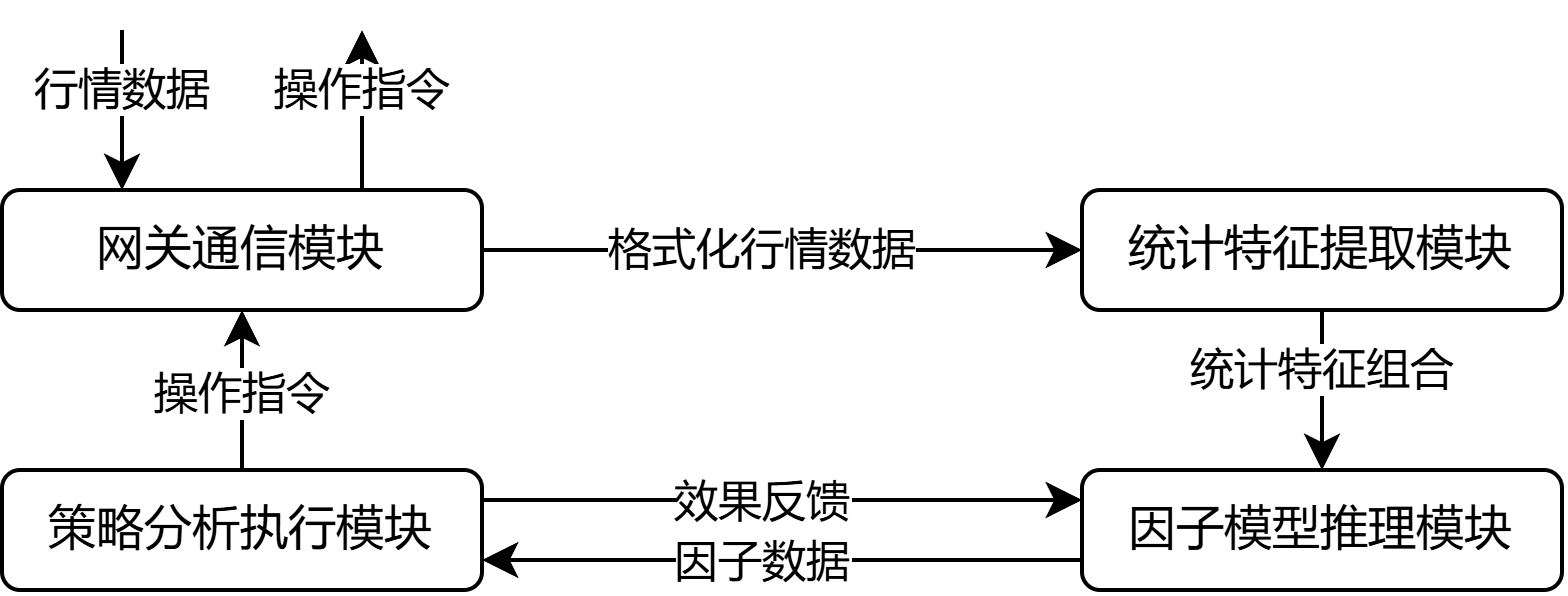
\includegraphics[width=1\textwidth]{image/chap02/lowlat.png}
    \caption{低延时交易系统基本架构}
    \label{fig:lowlatencysystem}
\end{figure}
低延时交易系统是量化交易的基础设施,其主要功能是在低延时的前提下完成市场行情的接收、分析与交易策略的执行。
如图\ref{fig:lowlatencysystem}所示,低延时交易系统以流水线的形式设计功能模块:
首先是网关模块,其负责接收和解析交易所的行情数据包,迅速将行情数据格式化后提交后续模块,确保数据实时与准确;
随后是数据预处理模块,接收格式化行情数据后更新内存数据库,然后对其进行清洗、标准化等操作,提取行情数据中的统计特征,为后续进一步分析提供基础;
接着是因子模型推理模块,该模块将预处理后的统计特征输入因子模型,然后执行计算推理,其输出作为对行情的表征;
最后是策略执行模块,依据因子模型的输出结果,决策和执行交易策略,向网关发送下单、撤单等操作请求,确保交易高效执行,同时向因子模型推理模块反馈信息。

为了实现高频交易下低延时的需求,低延时交易系统的设计与实现面临着诸多技术挑战。
整个交易流程关键路径的执行时间必须被严格控制在数十微秒之内,这对系统的每个模块都提出了极高的性能要求。
为此,交易系统中的各个模块均需要综合系统与硬件特性,从而尽可能提高系统执行效率,降低延时:
网关模块通过采用用户态网络库如DPDK甚至FPGA硬件加速技术,实现快速接收和解析行情数据;
数据预处理模块通过运用多线程并行处理与内存数据库如Redis以提高响应速度,或将模块编入内核态中完成数据清洗与标准化;
因子模型推理模块通过结合硬件架构调优算子,优化计算图与针对性的高效算法,显著降低模型推理延时;
策略执行模块则依赖高性能编程语言如C++和快速订单管理系统及直接市场接入(DMA)技术,以确保交易策略的高效执行。
在这一过程中,因子模型的推理计算尤其重要,由于其计算复杂度高,因此其推理延时在全过程延时中占有较大比例。
由此可见,提高因子模型的推理效率,降低其推理延时,就成为确保交易策略能够正确及时执行的关键所在。
这需要深入结合因子模型的结构特征,也需要对推理框架的架构设计和软件算法进行针对性的调整改进,以实现整个系统的高效运作。

\section{因子模型}

在低延时交易系统的运行过程中,因子模型推理模块通过将统计特征输入因子模型执行推理计算,从而向策略执行模块输出行情预测。
而因子模型作为量化交易行情表征的核心,设计的目标在于为行情建立模型,从中获取可用于策略分析的简易有效特征。
设计因子模型时,需从行情数据中挖掘出具有表征能力的特征因子,这些因子可以是行情基本面指标(如市盈率、市净率等),也可以是交易技术指标(如移动平均线、相对强弱指标等),也可以是宏观经济指标(如利率、通货膨胀率等)。
因子模型设计的最终目的在于通过统计和数学方法,建立因子与资产风险和收益间的定量关系,并借此探索因子影响资产未来收益的途径。


以公式\ref{con:inventoryflow}表示的动量因子为例,$\alpha_{i,t}$ 表示第 $i$ 个资产在时间 $t$ 的alpha因子值,$P_{t}$ 表示时间 $t$ 的资产价格,$P_{t-N}$ 表示时间 $t-N$ 的资产价格,$N$ 表示过去的时间窗口长度。
\begin{align}
    \begin{split}
        \alpha_{i,t} &= \frac{P_{t} - P_{t-N}}{P_{t-N}}, \\
    \label{con:inventoryflow}
    \end{split}
\end{align}
此类早期因子模型主要基于经验公式,直接对行情数据的某些统计量进行数学运算,一定程度上指示交易方向,但其表征市场行情特征的能力极其有限,难以应对复杂的市场环境。
尤其是伴随经验公式中超参数的引入,其调整难度和复杂性快速增加,实际应用价值逐步下降。
随着机器学习技术的发展,因子模型逐渐使用机器学习方法提高抗噪能力和表征水平。
现代因子模型,尤其是多分支因子模型,通过多分支结构综合处理多种行情指标,能够有效捕捉市场行情的复杂特征,极大提升了模型的表征能力和抗噪性能,为交易者提供了更为精准、可靠的决策依据,从而在激烈的市场竞争中占据优势。

多分支因子模型的输入通常是多种行情特征的拼接,在输入后切片进入不同的分支进行初步处理,随后通过计算操作融合各条分支,从而使得模型可以综合不同行情特征,并最终给出因子输出指示策略执行。
从输入模式方面,多分支因子模型的输入具有高度的可拓展性,其输入既包含了多个统计特征,但是又相互独立。
这使得多分支因子模型在计算过程相互独立的分支之间可以针对各分支输入实现优化算法。
在结构特征方面,多分支因子模型其整体结构类似树状收敛,分支之间融合后形成唯一的新分支,最终汇集为模型的唯一输出。
这种结构综合分析了多个分支的特征,有效提高了模型的性能,尤其是残差连接\cite{he2015deepresiduallearningimage}大幅提高了模型设计的可用深度,多分支因子模型因此具有更强的综合能力。
\begin{figure}[h]
    \centering
    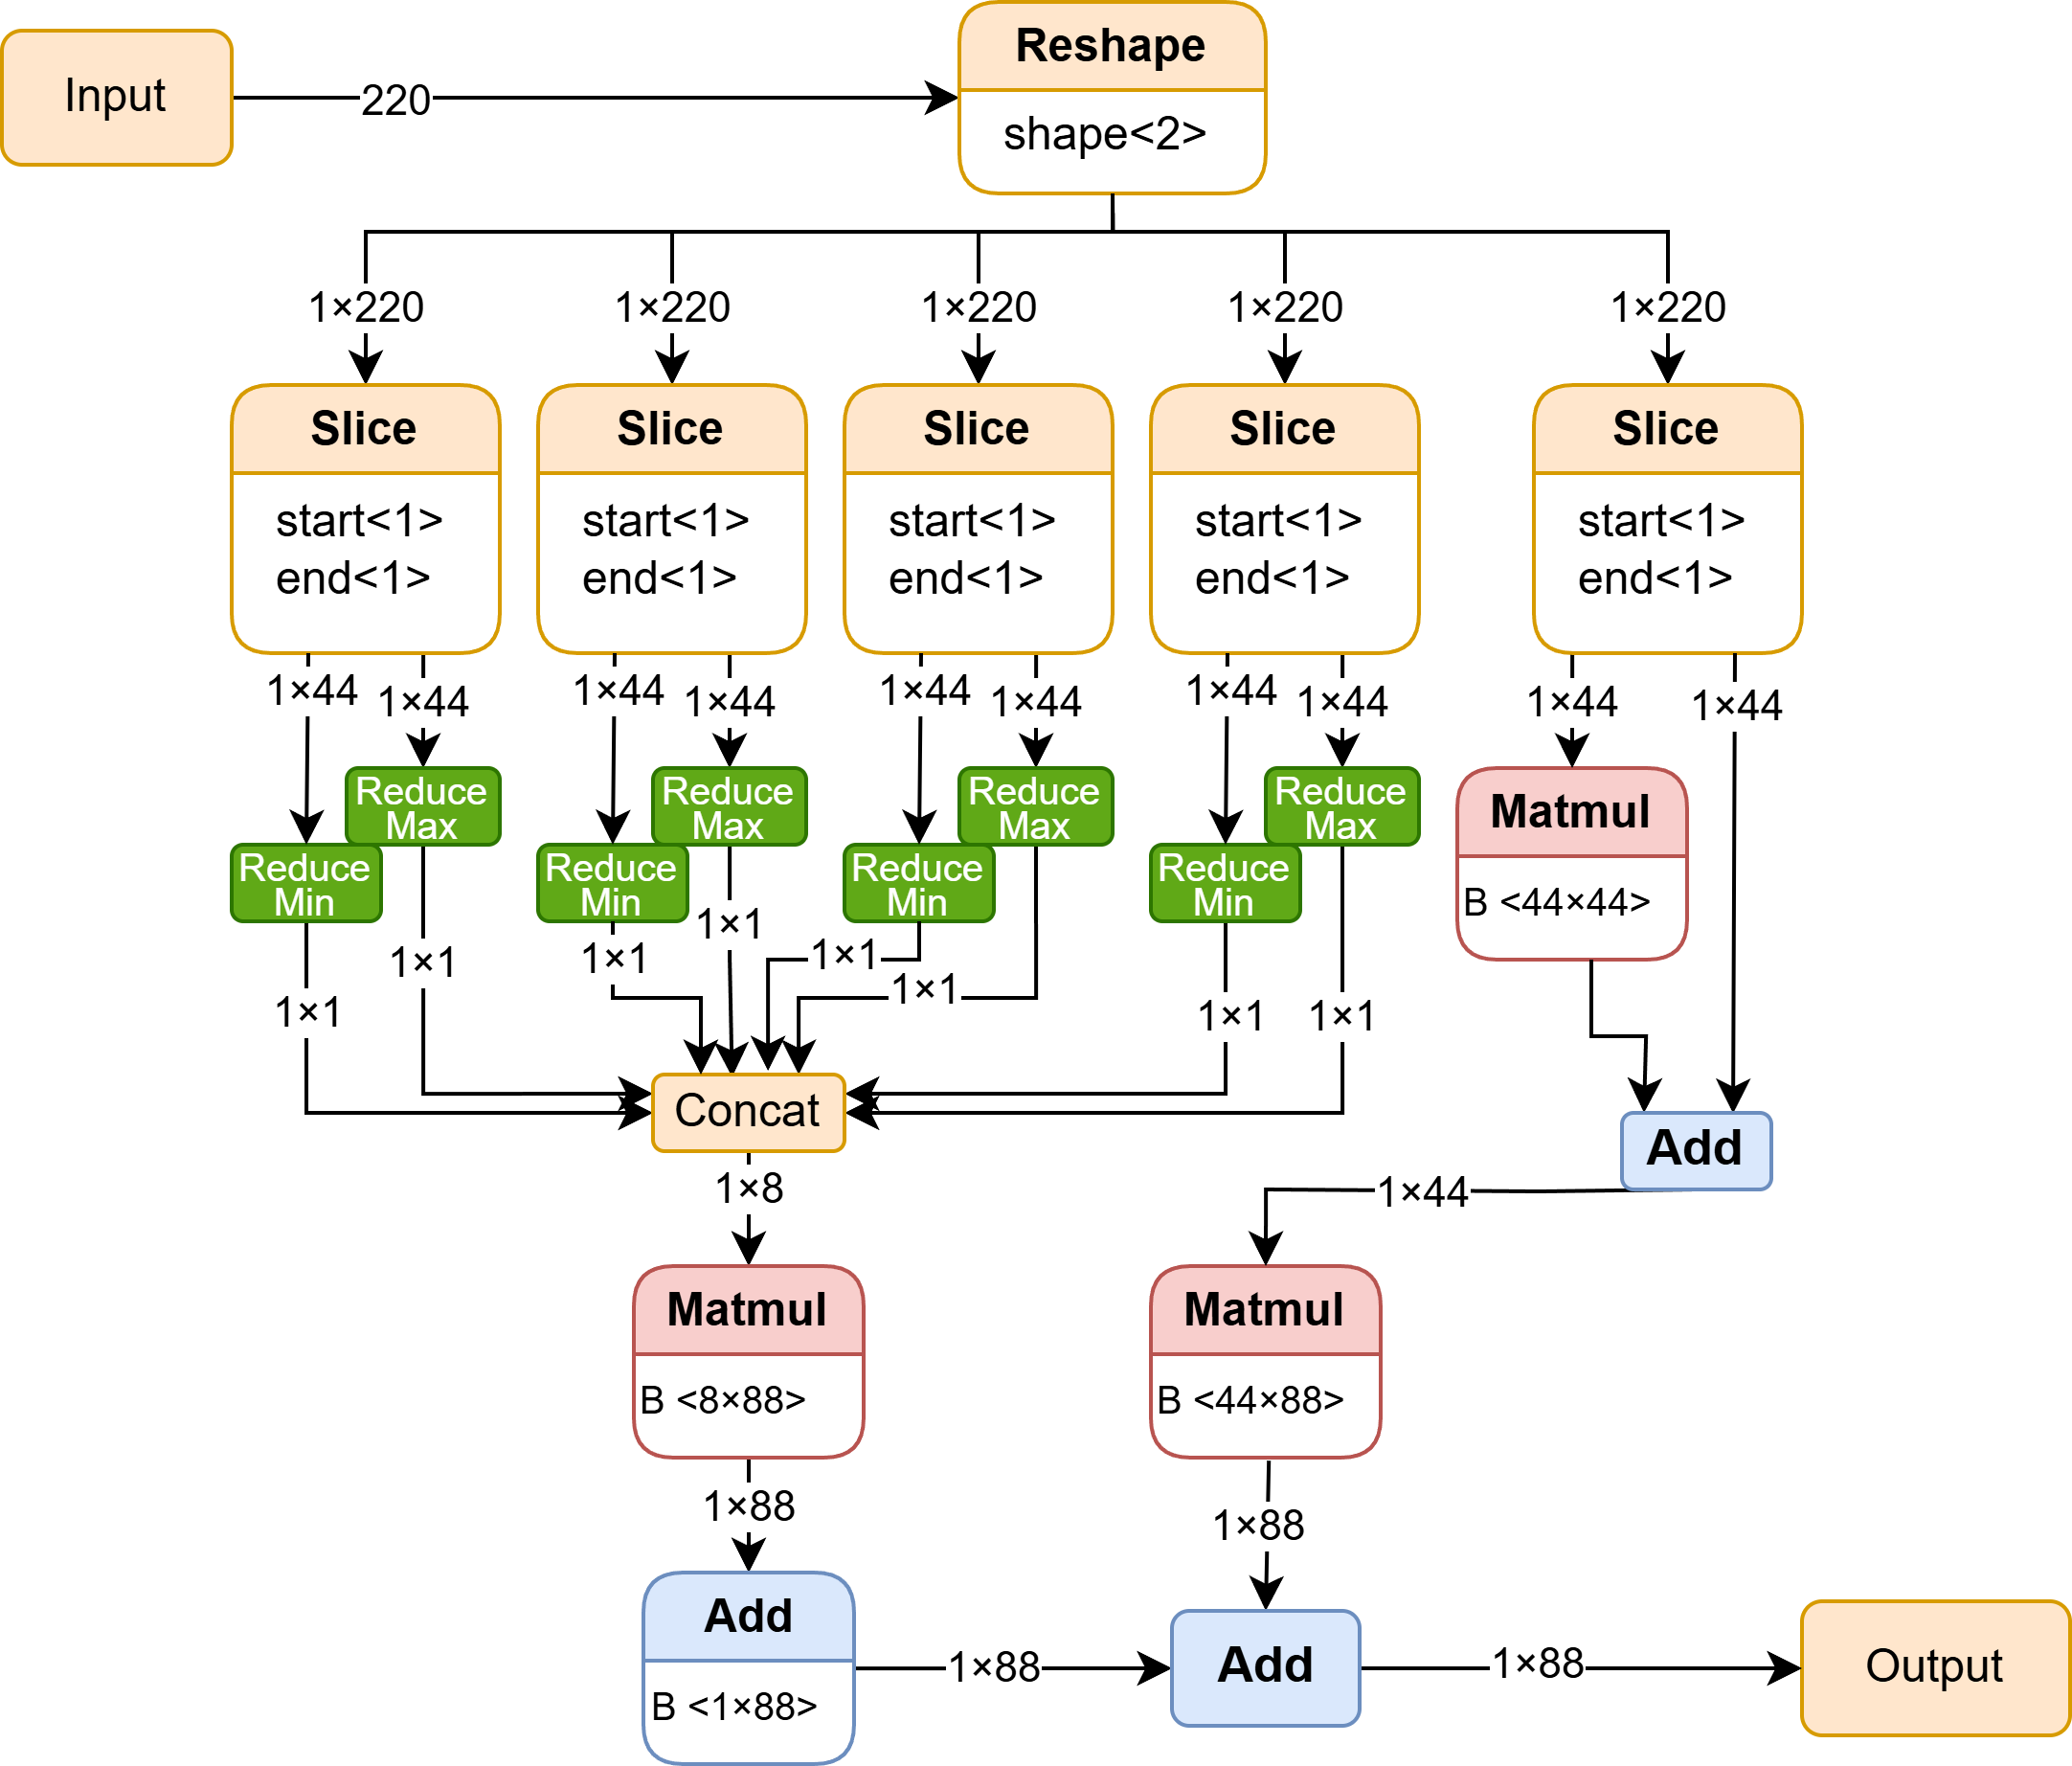
\includegraphics[width=1\textwidth]{image/chap02/models1.png}
    \caption{多分支因子模型样例}
    \label{fig:models}
\end{figure}


\section{模型推理框架}

在服务端高并发业务场景下,现有的多数推理框架侧重于处理大量请求的并行计算,通过分布式架构和异构计算来提高系统的吞吐量。
然而,低延时交易系统所面临的场景则截然不同,其优化的目标在于实现单样本高频率计算密集场景下的极低延时。
这就要求推理框架能够充分利用因子模型的结构特征与输入模式,通过针对性的优化策略,如内存映射、模型剪枝、算子融合等技术,有效提高模型整体的计算效率,降低推理延时。

当前多数模型推理框架仅针对服务端高并发场景进行了优化,对于高频交易的低延时要求缺乏针对性的解决方案。
然而即便优化的目的指标不同,现有推理框架的架构设计和技术应用对于低延时系统中的推理框架设计仍然具有参考意义。
例如,Tencent TFCC通过使用MLIR(多级中间表示)技术实现了自动算子融合,极大减小了由于算子编码调优而浪费的时间和人力,并显著降低了推理延时,
同时基于MLIR的优化路径机制具有极强的可拓展性,优化路径之间彼此解耦合,具有极高的优化上限。
llama.cpp则作为一个高度优化的C/C++实现,专注于本地LLM推理性能的优化,充分利用了现代CPU架构中的SIMD指令集,为多个LLM工具和应用提供了基础运行时支持,
其使用Protobuf作为模型的解析器,通过C++将模型进行进一步的包装和抽象,拓展了模型结构,同时为进一步优化提供开发空间。
TensorRT是NVIDIA推出的一个高性能深度学习推理优化模块和运行时引擎,其包括静态计算图优化和动态推理优化两个解耦合的基本过程,
其静态计算图优化过程向上对模型适配,而动态推理优化过程向下对硬件适配,取得了优异的性能。

除了现有模型推理框架的架构设计和技术应用外,因子模型的推理框架还应当面向系统和硬件做出针对性优化。
例如,在推理的执行过程中,缺页中断将导致严重的延时增长,因此使用大页的内存映射和内存锁定方法,能够在系统运行全过程内不发生缺页中断,有效提高访存性能。
利用系统调度指定CPU核心隔离操作,可以尽可能减少无关进程在指定核心的运行,从而有效提高CPU的占用时间。
在这些推理框架中,面向硬件的优化也是一个关键环节。
在日志系统的计时过程中,使用rdtscp指令计数器参与计时,能够以多核一致性clock的细粒度进行计时,完成高精度的性能测试。
通过针对特定硬件架构的算子实现,可以充分利用硬件的并行计算能力,提高计算效率。

总体来看,在模型推理框架的整体设计上,应当效仿先进的架构设计和技术应用,这将有效提高优化手段的效果上限。
同时在具体的内存管理和系统配置等方面,也要充分利用相关系统属性进行优化以提高访存和计算效率。
只有在综合多种优化手段的前提下,模型推理框架才能够在高频交易的低延时环境下有优越的性能表现。

\section{高频交易下CPU计算架构}

尽管当前模型推理的硬件设备以GPU为主,但以业内普遍使用的英伟达A100计算卡为例,从CPU发起空核函数到GPU执行核函数之间的延时就高达2.59微秒,而连续空核函数之间的间隔延时约为5微秒。
而在更早的特斯拉架构中,发起矩阵乘操作核函数,其间隔延时高达20微秒,使其不具有应用价值。
\begin{figure}[h]
    \centering
    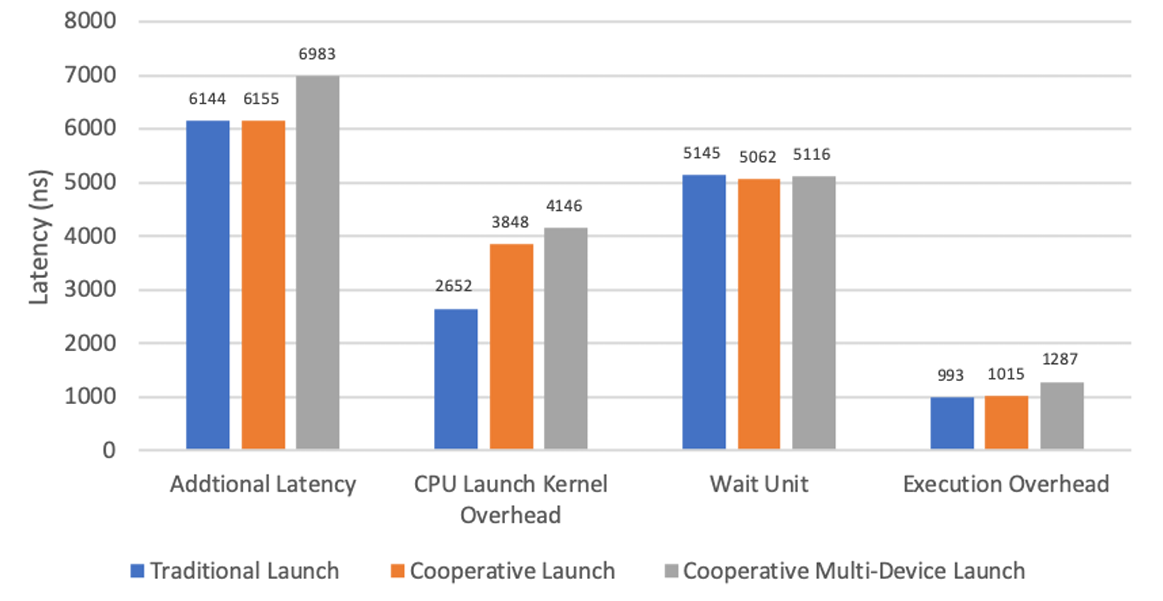
\includegraphics[width=1\textwidth]{image/chap02/Overhead.png}
    \caption{使用不同方法发射大型核函数的执行延时组成}
    \label{fig:kernelss}
\end{figure}
如图\ref{fig:kernelss}所示,图中Traditional Launch,就是CUDA程序中常用语法糖发射的接口;
Additional Latency代表额外的延迟,是CPU刚刚调用了一个发射核函数后发射另一个核函数的额外延迟;
CPU Launch Kernel Overhead代表CPU调用发射函数到GPU执行的延迟;
Wait Util是核函数的内容,测试过程中通过多次调用Wait定时函数来填充核函数;
Execution Overhead指GPU的实际执行时间和Wait定时函数执行时间的差值。
可以观察到,在加入参数和数据传输后,延时已经使得因子模型在以期货市场为核心的高频交易中失去竞争力。
此外,尽管在多数工程计算场景如有限元计算中,计算过程通常被整体编码为一个核函数,
但对于时刻变化的业务模型,包括交易因子模型在内,为了维持项目的可读性和可维护性,不可避免地对计算节点进行抽象,进而将整个模型抽象为一个由算子组成的计算图。
在这种抽象计算图的推理过程中,算子核函数的连续发起导致仅累计启动延时就已超出预期。
因此,因子模型推理的目标硬件普遍使用服务器高性能多核CPU,尤其以AMD EPYC和Intel Xeon为业务主流硬件。


\begin{figure}[h]
    \centering
    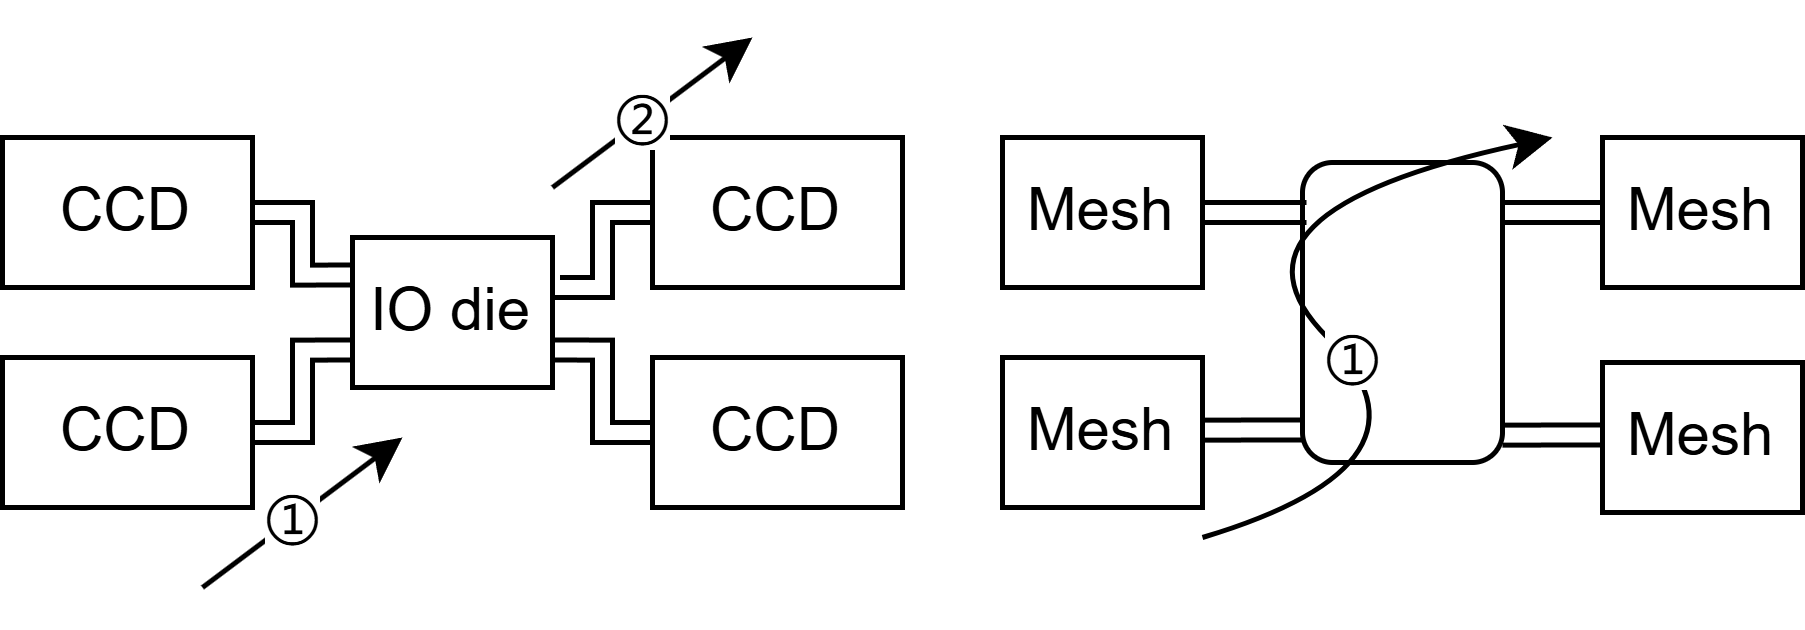
\includegraphics[width=1\textwidth]{image/chap02/arch.png}
    \caption{AMD EPYC与Intel Xeon在CPU NUMA访存过程对比}
    \label{fig:cpus}
\end{figure}

在高频交易场景下,CPU的架构特性对因子模型的实际推理模式和效率有显著的影响,为此,优化方案需要围绕如何提高CPU利用率来设计开发。
现在主流的CPU架构里,AMD EPYC和Intel Xeon在多核的拓扑封装方面存在着显著的差异,如图\ref{fig:cpus}所示:
AMD EPYC架构基于CCX和CCD的核簇模式设计,在单个核簇内多个核心共享L3缓存,借助核簇内的高速通信总线和大L3缓存,相比较Intel Xeon在多线程、大规模数据的计算场景下具有显著的性能优势。
Intel Xeon在拓扑封装方面则采用环路架构,核心间通过环形总线通信,相比AMD EPYC,通信延时明显下降,其在单线程性能和跨核访存方面具有优势,
能快速处理高频率单样本的计算任务,更符合低延时交易系统需求。同样在高频交易中常用的一读多写场景中,其广播延时和多播延时比AMD EPYC有明显的改善。
如图\ref{fig:cpus}所示,AMD EPYC处理器在跨核心访存过程中相比较Intel Xeon处理器存在路由的中间过程,而在多个业务实例部署且跨核通信密集的场景下,IO die的路由效率极其有限,这直接导致AMD EPYC相较于Intel Xeon有更高的一致性延时。
除了拓扑封装的差异导致跨核通信的性能差异外,两者在指令集支持上也有诸多不同,这也决定了它们在不同计算场景下的适用性。
Intel Xeon在支持AVX512指令集方面表现出色,而AMD EPYC在连续数个版本只使用AVX2模拟AVX512来实现指令集兼容。
因此,对于某些SIMD高需求的应用如向量数据库,AMD EPYC的计算性能就略显不足。
综上所述,框架实际的优化方案必须结合具体业务场景和CPU架构特性以设计实现,如此才能达到最优性能。
充分利用不同CPU架构的特性,是改善推理过程延时的关键。

为了把CPU的计算能力发挥到极致,目前已有多种高性能计算库针对不同CPU架构实现针对性性能优化。
以Intel MKL和AMD AOCL为例,其分别为Intel Xeon和AMD EPYC处理器提供高效的计算操作接口。
通过调用常用的BLAS操作接口,开发者能够迅速实现对目标应用的性能调优。
Intel MKL GEMM JIT是Intel MKL推出的专注于小规模矩阵乘的高效计算接口,
通过即时编译技术生成针对特定矩阵尺寸和数据类型的高效计算代码,从而提升矩阵运算性能。
Blaze HPC是个高效的数值计算库,在算子调优的流水线中,通常作为最后一级编译输出的部分,通过将已完成设备指令集适配的BLAS传入Blaze HPC,
然后向其配置文件写入CPU的指令集和各级缓存信息,算子即可实现细粒度的自动调优以实现最优性能。
它通过高度优化的算法和数据结构,有效提高CPU计算的利用率,加速数值计算过程。
Blaze HPC还支持张量运算,为因子模型推理框架提供了基本的高性能算子实现,让CPU在高频交易场景下能高效完成复杂计算任务。
\newclearpage
\chapter{多分支因子模型推理框架方案设计}

高频交易场景下对模型的单样本推理过程有严苛的低延时要求,针对多分支因子模型的模型结构和业务场景的计算要求,本文提出了多分支因子模型推理框架。
本章将首先详细阐述多分支因子模型推理框架的总体设计方案,讲述框架的架构设计和基本功能,
随后针对高频交易场景中业务需求的单样本,低延时,多分支等特点,从内存管理和系统配置、算子调优与绑定到分支优化加速的角度更细粒度地介绍优化方法和加速算法设计。
\section{总体设计方案}

因子模型的部署推理过程可以被抽象分为静态预处理和动态运行两个紧密关联且分工明确的阶段。
\begin{figure}[h]
    \centering
    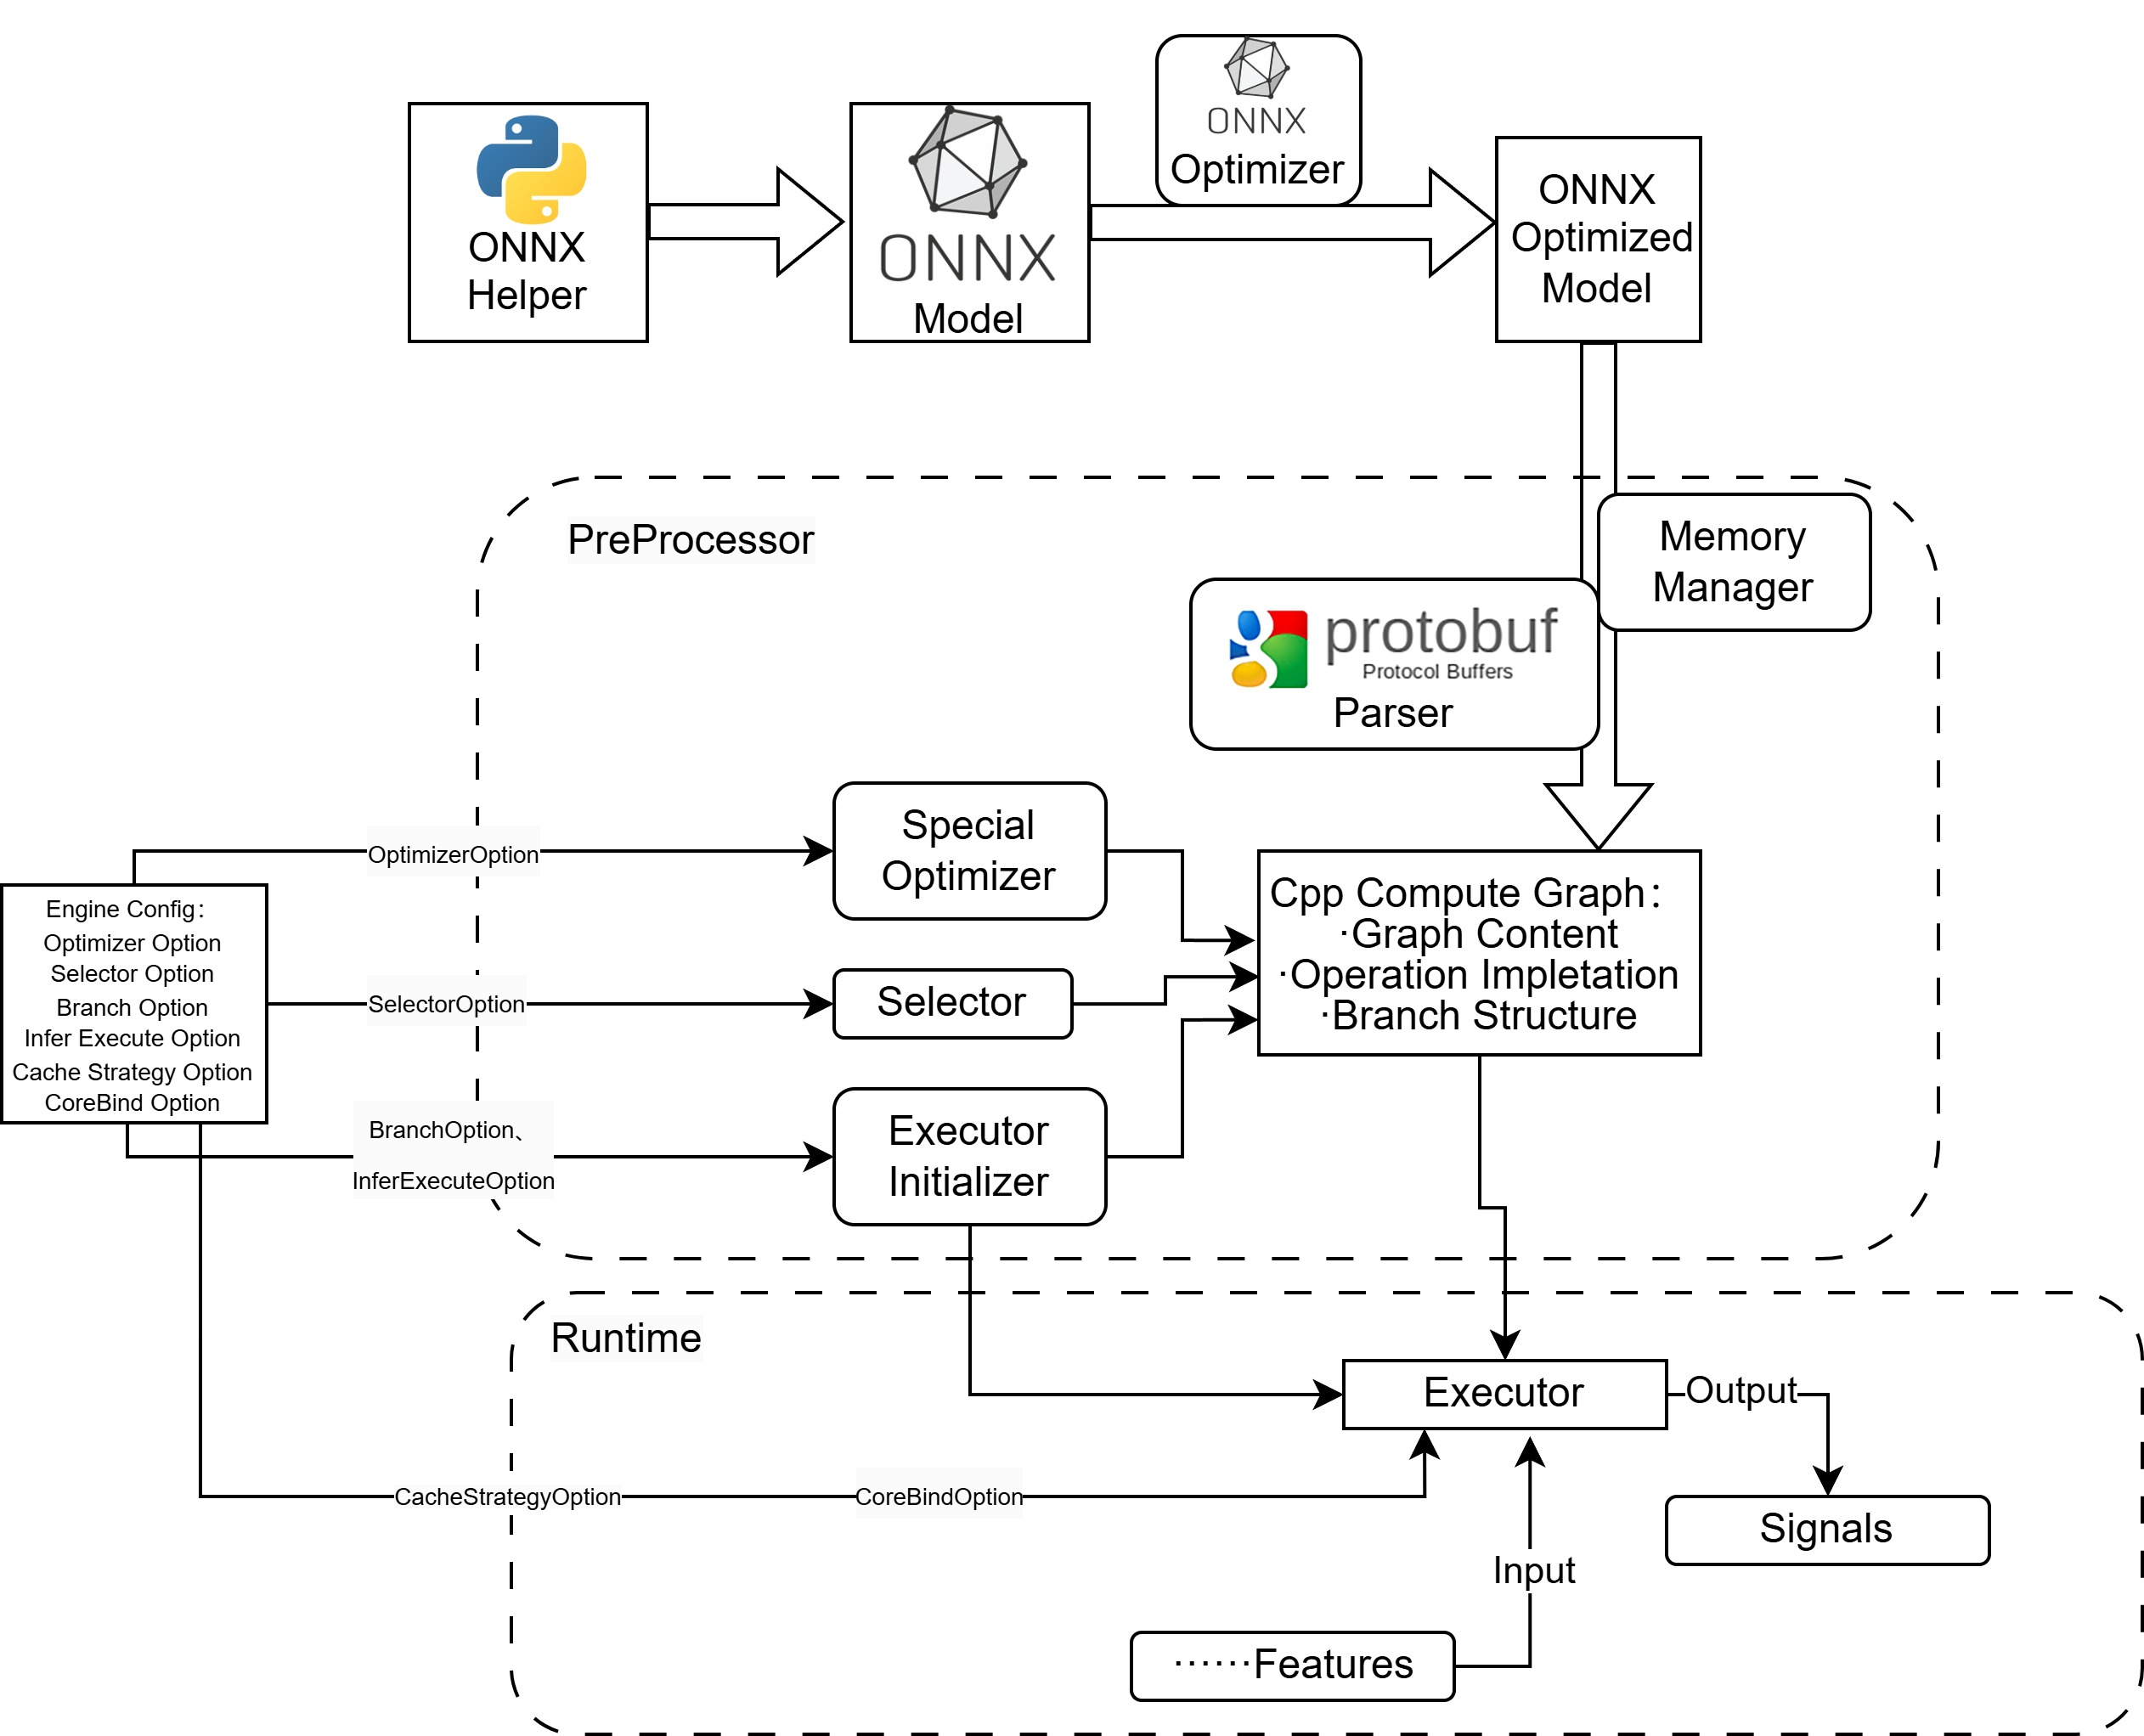
\includegraphics[width=0.9\textwidth]{image/chap03/framework.jpg}
    \caption{框架整体设计}
    \label{fig:hole}
\end{figure}

静态预处理阶段,其核心在于重建计算图并进一步实施多方面的优化。
在此阶段,通过采用Protobuf的高效序列化工具,能够将ONNX格式的机器学习模型解析并映射到C++类对象结构中。
这一过程不仅确保模型数据结构完整可用,也为后续优化操作提供对象基础和拓展空间。
在实际的优化流程中,研发人员依据既定的优化目标和需求,可以选择性地引入各类Pass。
例如,无效算子消除Pass能够识别并删除对模型最终输出结果无贡献的算子节点,从而有效简化计算图的结构;
算子融合Pass将多个在逻辑上紧密相连、在功能上可整合的算子进行合并,以此减少推理过程中的冗余访存和计算开销,提升计算资源的利用效率;
模型剪枝Pass通过去除模型中相对冗余的连接或节点,实现模型规模的削减,在不显著影响模型性能的前提下降低存储和计算负担;
量化Pass则专注于将模型中的高精度数据类型转换为低精度类型,从而在保证模型性能基本稳定的前提下,进一步提升计算效率,降低硬件资源的占用。
通过Optimizer中Pass的执行,推理框架能够像编译器一样对计算图独立开展优化,产生相对垂直的优化效果。
此外,静态预处理阶段还包含算子对硬件环境的适配与调优过程,能够基于目标设备的硬件配置细节,包括处理器架构、内存容量、缓存大小等关键参数,并依据这些信息对计算图中的各个算子进行针对性的调优和加速。
针对不同架构的处理器,可以优化算子的指令集使用,充分利用硬件的并行计算能力和缓存机制,以实现计算性能的最大化。
同时,本文提出的因子模型推理框架在静态预处理过程中,会基于配置请求预先完成分支分割和缓存算法等关键机制的基础设置。
其中,分支的拓扑分割操作依据模型的结构特点和运行需求,将复杂的计算图划分为多个相对独立且易于处理的子图分支,为后续的缓存应用和资源分配提供便利。

动态运行阶段则侧重对静态预处理之后所形成的各个组成部分进行高效的动态加载与运行。
在此过程中,核心隔离和绑定操作能够确保模型的不同部分在计算资源上实现合理分配与高效利用,避免资源冲突和浪费。
具体而言,通过将不同的计算任务绑定到特定的处理器核心或线程上并将核心隔离,可以使得极大减少由于系统进程调度导致的性能损失。
同时,分支缓存机制能够根据实际运行时的数据流情况,快速调整分支计算策略,保障模型运行保持高效。

综上所述,因子模型推理框架通过科学合理地结合静态预处理与动态运行这两个阶段,实现了局部优化与整体调度的协同提升。
这种将两者相分离的设计方案,在工程设计上降低了项目开发复杂度,为后续的优化工作开拓空间。
以此本文能够在此基础上,探索实现更多优化策略,推动因子模型推理性能提升,以适应日益复杂和多样化的应用场景需求。

\section{内存管理方法}

在高频交易场景下,多分支因子模型推理框架的运行依赖于高效的内存管理策略。
为了满足低延时的要求,推理框架采用了内存池(Memory Pool)和分配器(Allocator)相结合的内存管理机制。
这种机制通过预先分配大块内存并按需分配给计算图节点,显著减少了动态内存分配带来的延时开销,同时提高了内存使用的效率和稳定性。

内存池是推理框架内存管理的核心组件,其主要功能是预先分配一块大容量的内存空间,并在推理过程中按需分配给各个计算节点。
为了最大化内存访问速度并减少内存碎片化,内存池使用了mmap系统调用分配一个基于Huge Page的1GB内存区域。
Huge Page是一种操作系统提供的大页内存管理机制,通过减少页表项的数量,降低内存访问的TLB(Translation Lookaside Buffer)缺失率,从而显著提高内存访问速度。
在初始化阶段,推理框架通过mmap调用请求一个1GB的Huge Page内存区域,并将其映射到进程的地址空间。
这块内存被划分为多个固定大小的内存块,每个内存块对应一个计算图节点的内存需求。
内存池维护一个指针,指向当前可分配内存的起点。每次分配内存时,内存池通过更新该指针的位置来分配连续的内存块,从而避免了传统动态内存分配算法中的锁竞争和内存碎片化问题。
内存池的设计还有助于提高系统的可扩展性,便于根据不同的硬件配置和应用场景进行灵活调整,确保在不同环境下都能实现最优的内存管理效果。

内存分配器是内存池的管理接口,负责将内存池中的内存分配给具体的计算图节点。
在推理框架的预处理阶段,计算图的每个节点会根据其输入和输出张量(Tensor)的大小向分配器请求内存。
分配器根据节点的请求,从内存池中分配相应的内存块,并将内存的起始地址返回给节点。
在张量初始化时,推理框架会根据张量的形状和数据类型计算所需的内存大小,并通过分配器从内存池中申请内存。
分配器会检查内存池中是否有足够的连续内存块可供分配。
如果有,则更新内存池的起点指针,将内存块分配给张量;如果没有,则返回错误。
分配器还具备智能分配策略,能够根据节点的优先级和内存需求的紧急程度,合理分配内存资源,确保关键节点的内存供应,从而进一步提升系统的整体性能和可靠性。
此外,分配器在内存回收方面也进行了优化,对于不再使用的内存块能够及时释放并归还给内存池,以供其他节点重新使用,进一步提高了内存的利用率。

为了进一步优化内存管理的性能,推理框架在初始化结束后固定已分配的内存区域。
这一策略基于高频交易场景下模型输入和输出张量大小相对固定的特点。
在初始化阶段,推理框架会一次性分配足够的内存。一旦初始化完成,内存池中的内存分配便不再变化,从而避免了运行时的动态内存分配和回收操作。
此外,推理框架还通过内存锁定机制(Memory Locking)将分配的内存锁定在物理内存中,防止操作系统将这些内存页交换到磁盘。
这不仅减少了内存访问的延迟,还提高了系统的稳定性,确保在高频交易的高负载场景下不会因内存交换而引入额外的延时。
这种固定的内存分配策略还有助于提高系统的可预测性,便于对内存使用情况进行监控和优化,为系统的长期稳定运行提供有力保障。
同时,通过固定内存区域,可以有效减少因内存分配和回收频繁操作而导致的系统开销,使得推理框架能够更加专注于模型的计算和推理任务,从而在高频交易中快速响应市场变化,做出精准的交易决策。

\begin{figure}[h]
    \centering
    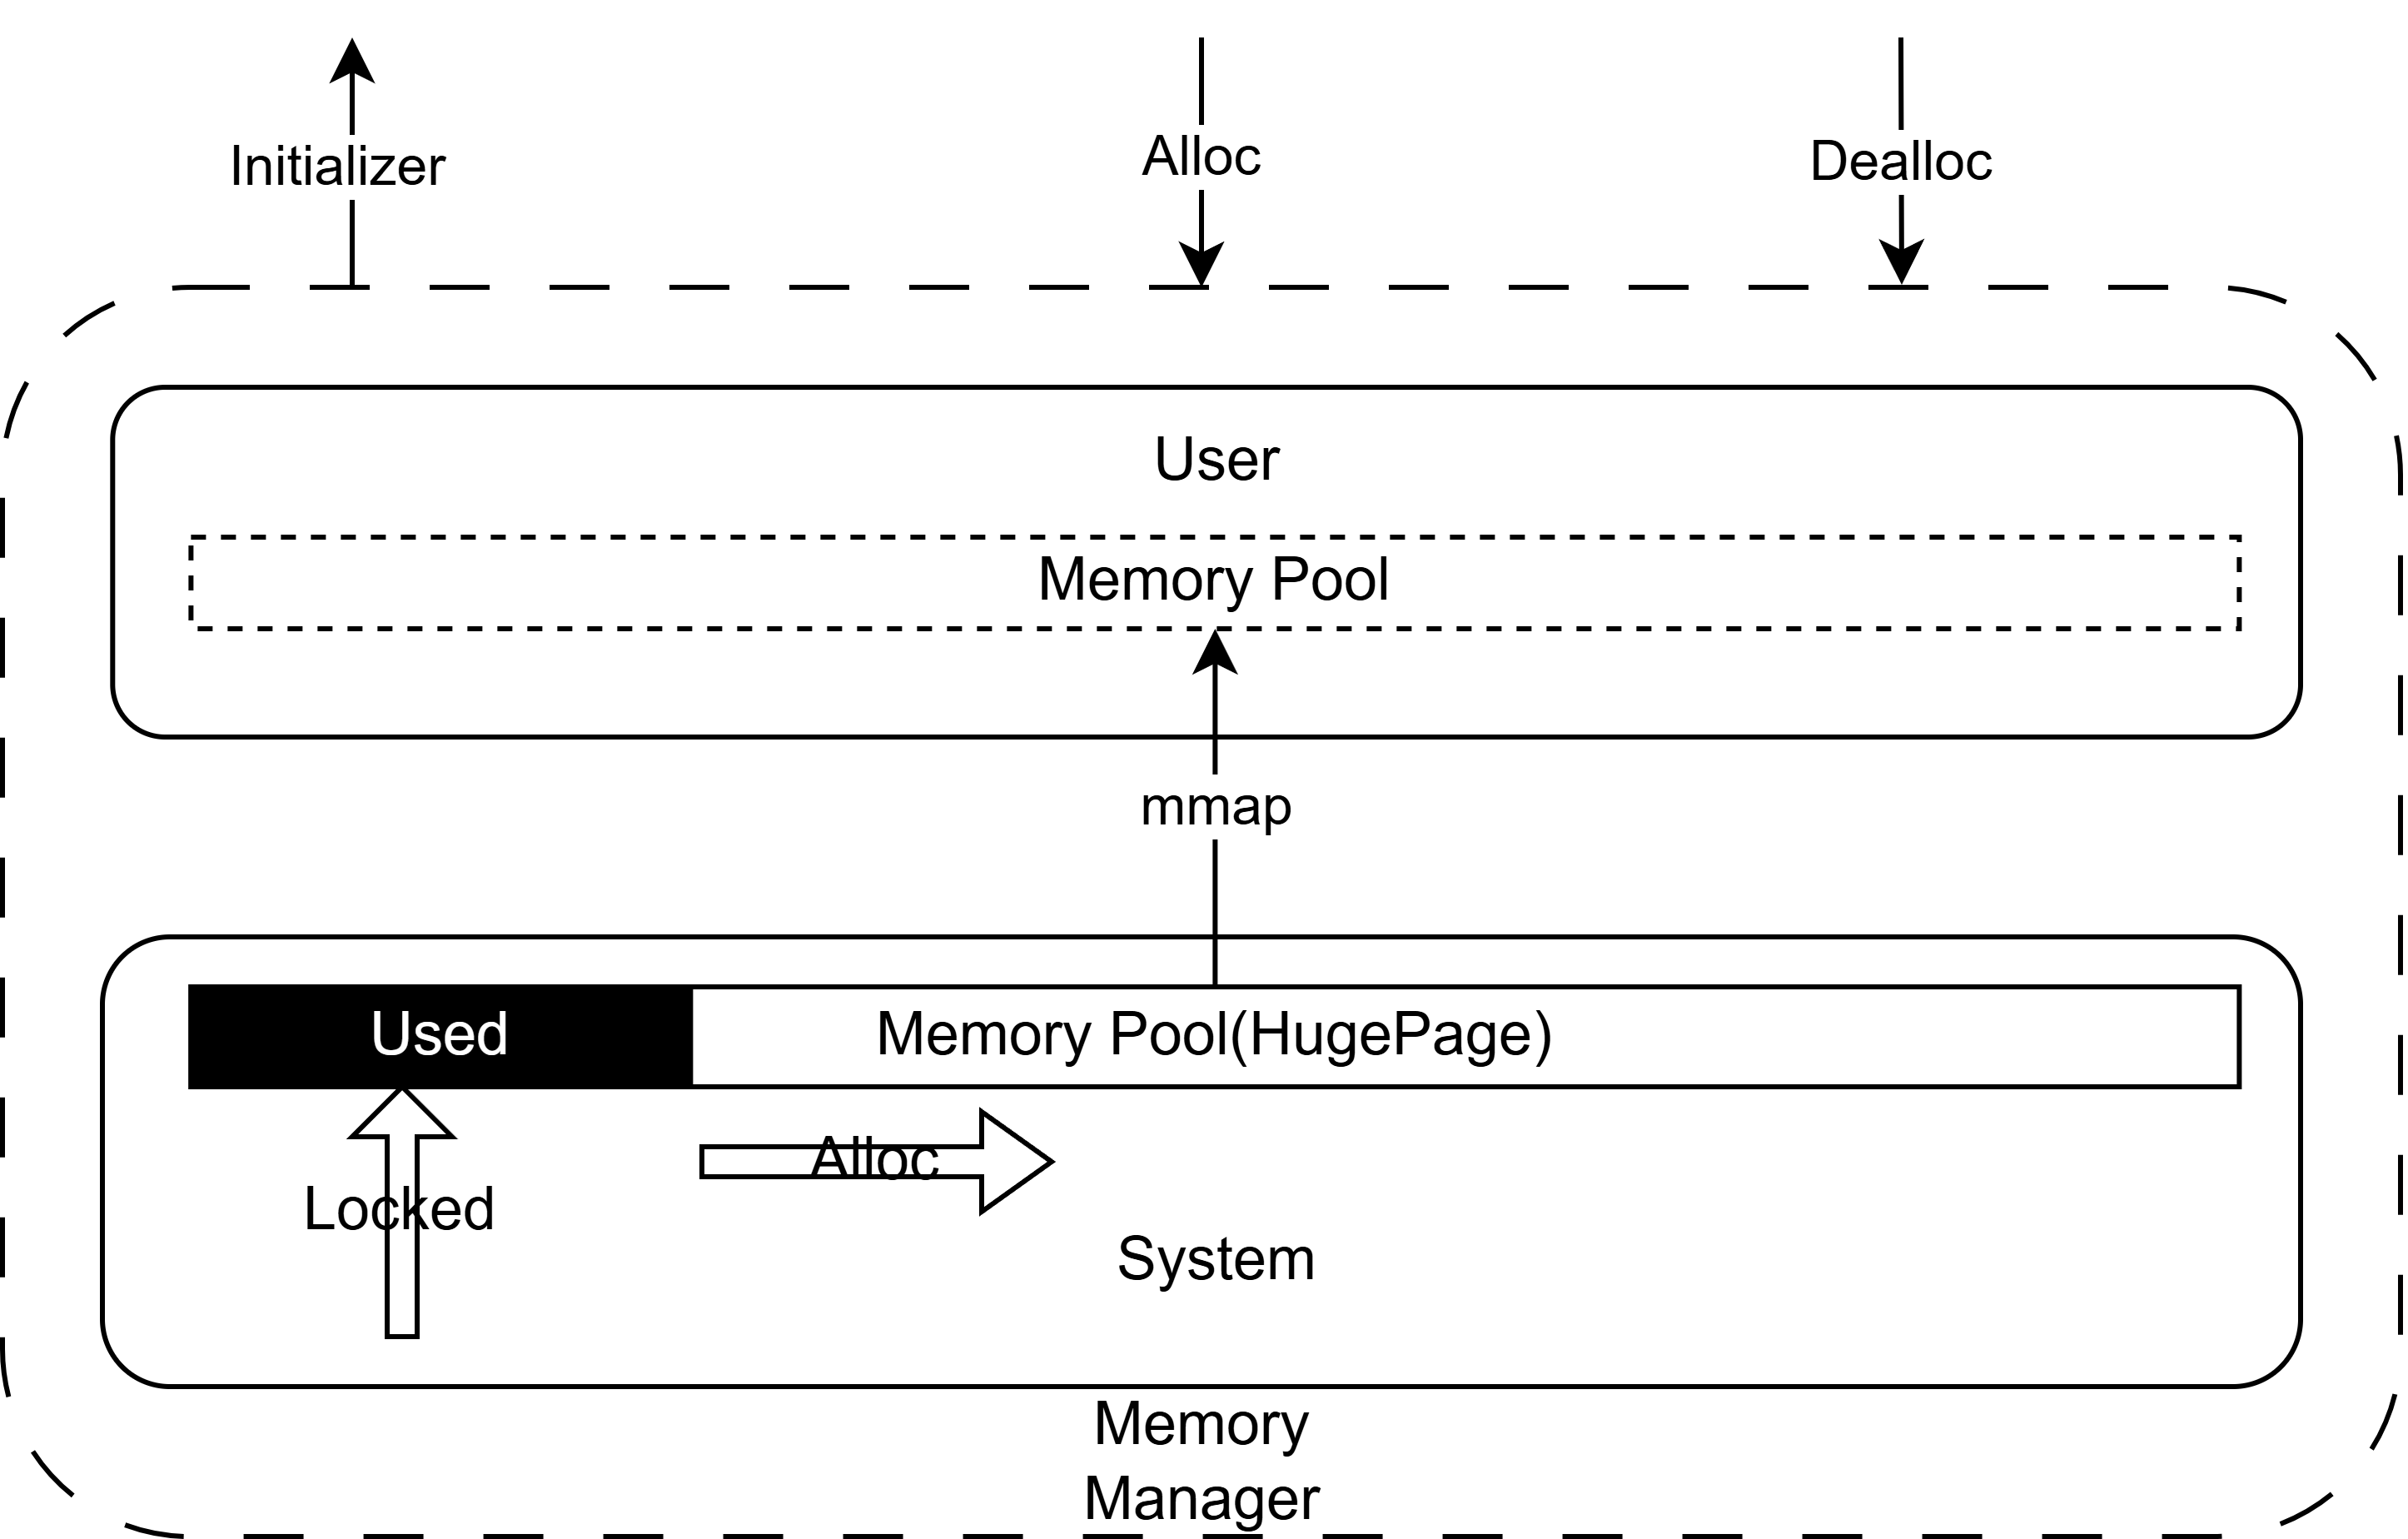
\includegraphics[width=0.9\textwidth]{image/chap03/memmory.png}
    \caption{内存管理器}
    \label{fig:hole}
\end{figure}

推理框架的内存管理机制通过内存池和分配器的设计,结合Huge Page和内存锁定技术,有效解决了高频交易场景下低延时和高效率的内存管理需求。
这种机制不仅减少了动态内存分配的开销,还提高了内存访问的速度和稳定性,为高频交易中的多分支因子模型推理提供了强大的支持。
在实际应用中,该内存管理机制能够显著提升推理框架的性能表现,使其在高频交易领域中具备显著的竞争优势,能够更有效地处理大规模数据和模型推理任务。

\section{算子调优与绑定}
在高频交易业务场景下,程序自动交易链路的全过程对延时的要求极为苛刻,关键路径的最大延时必须被约束在数十乃至数微秒。
这一延时标准直接决定了量化策略是否能够在指定价格位置准确执行交易,否则可能导致显著的损失。
因此,作为关键路径中延时的主要来源,因子模型的计算过程必须充分利用硬件性能以减小延时,其中算子的调优是至关重要的环节。

在此前提下,框架提供了算子调优与绑定的简易步骤,加速了框架应用于目标硬件的部署实践。
首先,框架在Blaze HPC编译过程中结合Intel MKL、AMD AOCL等数学库与CPU架构信息,如各级缓存大小、指令集等,从而在算子性能本身提供最优实践。
其次,对于Blaze HPC不支持的进一步优化,在部署框架过程中,框架通过Selector类可以综合计算需求和CPU信息来动态绑定算子。
例如,Intel GEMM JIT对于小规模浮点数矩阵乘有显著加速效果,框架通过判定指定节点的计算类型和规模,可将该节点算子绑定到Intel GEMM JIT。
因此,算子绑定过程具有极大的可拓展性,对于先进的计算优化也可以通过简单的拓展开发进行快速适配。
同样,模型经过静态优化器可以产生节点的融合,对于此类非常规的算子,BLAS通常不能提供支持,但框架仍然支持通过简易的拓展开发实现手写算子,只需要使用CPU定制编译器如ICPX等进行目标架构的针对性优化即可。
通过上述算子的调优与绑定过程,算子执行得以充分利用硬件的性能,极大提高了因子模型的推理效率。

具体到指令集覆盖方面,在CPU算子优化过程中,充分利用现代CPU的指令集和架构特性是提高性能的关键。
特别是AVX2和AVX-512指令集,它们能够显著提升数据的并行处理能力。
AVX2支持256位的向量化操作,而AVX-512则进一步扩展到512位,理论上能够提供更高的计算效率。
然而,在实际应用中,AVX-512的性能提升并不总是显著的,尤其是在某些特定型号的CPU上。
例如,对于AMD EPYC系列CPU,虽然其支持AVX-512指令集,但在某些场景下,使用AVX-512可能会导致CPU积热,从而触发降频机制,反而降低了整体性能。
为了避免这种情况,优化策略中需要根据具体的CPU型号和应用场景灵活选择指令集。
例如,在AMD EPYC平台上,可以优先选择AVX2指令集,以避免因积热导致的降频问题。这种策略不仅能够保证CPU在高频交易场景下的稳定运行,还能充分利用硬件的计算能力。

在实际的交易场景中,这种优化策略的实施包含多个过程。
首先,需要对不同的CPU型号进行详细的性能测试,以确定在特定工作负载下哪种指令集能够提供最佳的性能表现。
这既包括对不同指令集在矩阵运算、浮点运算等常见计算任务中的执行时间、能耗以及温度变化的监测,
又要考虑交易系统的整体架构,包括数据传输、任务调度以及与其他系统组件的交互,确保算子优化不会引入新的瓶颈。
通过针对硬件性能的细粒度优化,可以确保高频交易系统在市场竞争中保持性能优势,实现高效的交易执行和风险控制。
\section{分支拓扑分割算法}
\begin{figure}[h]
    \centering
    \includegraphics[width=0.9\textwidth]{image/chap03/branchs.jpg}
    \caption{分支拓扑分割算法中以分支为单位的计算图重建}
    \label{fig:hole}
\end{figure}
在量化交易中,多分支因子模型被广泛应用以生成交易信号。
这些模型的输入通常由多个市场特征拼接而成,这些特征在前序步骤中经计算操作,进入模型后被切分到不同分支中处理。
尽针对管不同交易品类所设计的多分支因子模型在具体设计上存在较大差异,
但整体上,各个分支在经过一定处理后,都会通过通用矩阵乘法(GEMM)映射到高维空间,然后各分支之间通过计算操作逐级合并,最终得到一个输出。
从形状上看,这种模型结构类似于一个从叶子到根的树状收敛结构。
\begin{wrapfigure}{r}{0.4\linewidth}
    \centering
    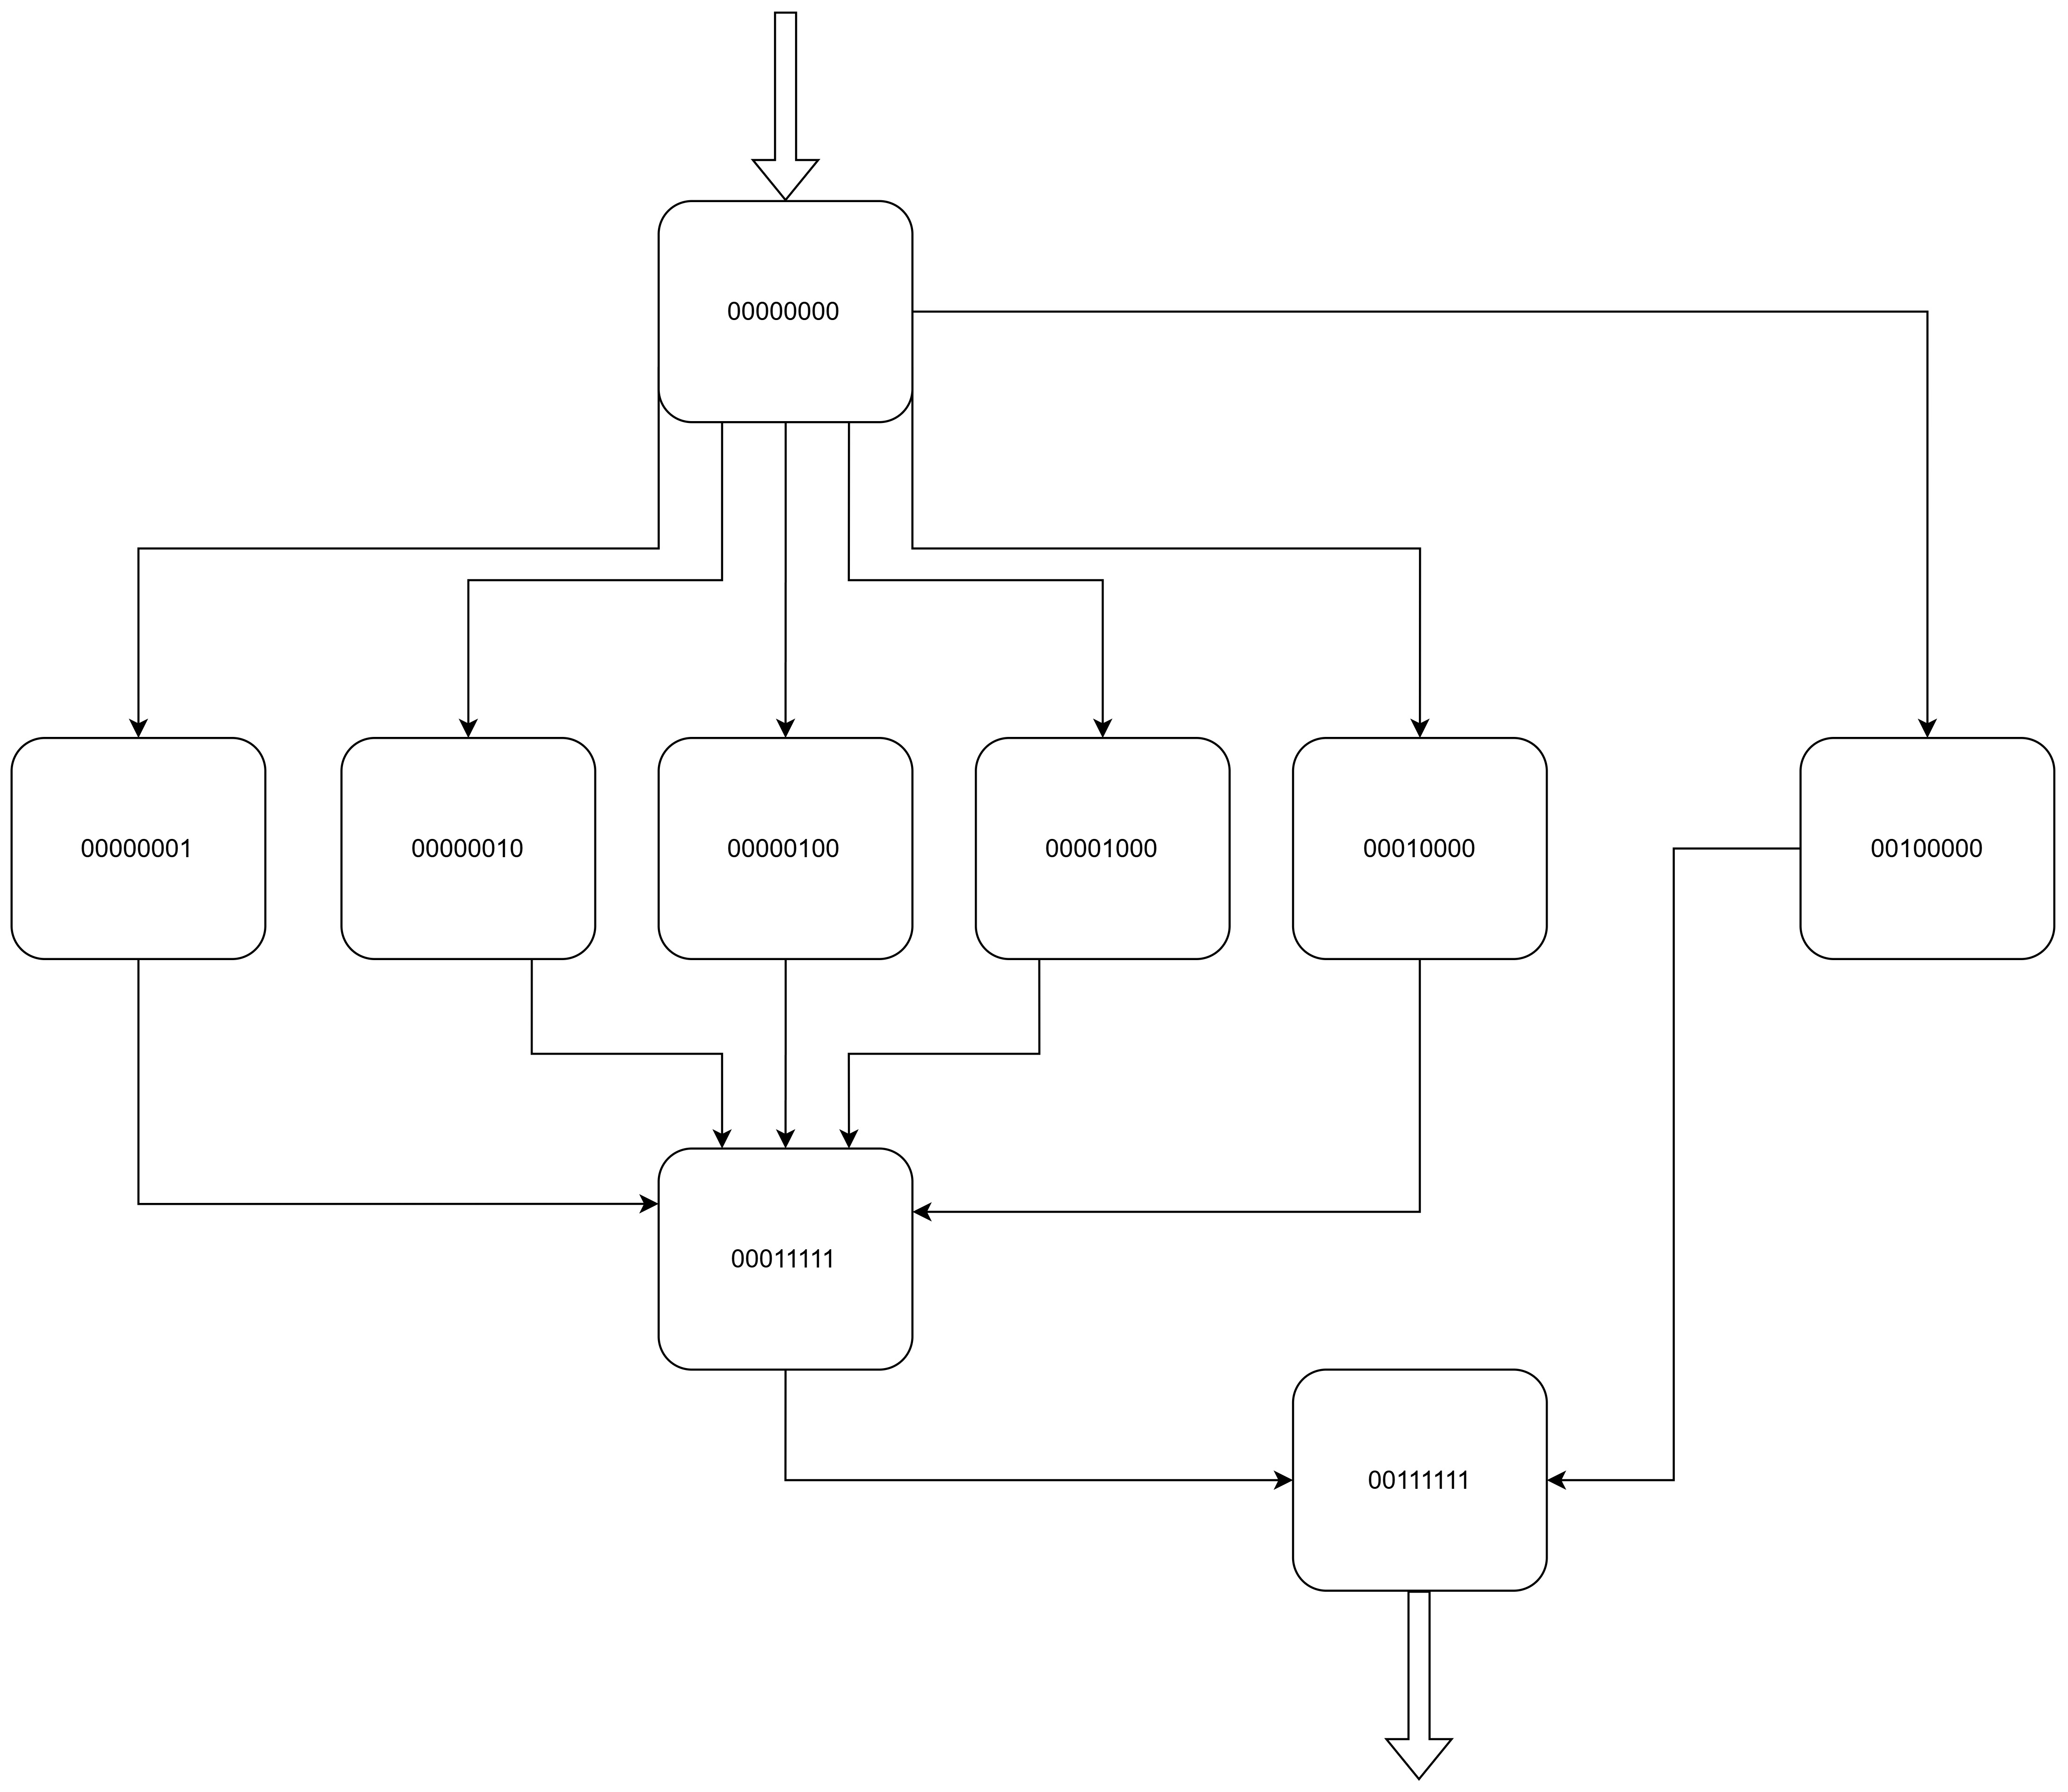
\includegraphics[width=0.4\textwidth]{image/chap03/branch2.jpg}
    \caption{分支位标记示意图}
    \label{fig:image-embedding-text}
\end{wrapfigure}
为了优化模型的推理过程,我们利用位运算来标记各个分支,
并通过这种方式,将以节点为单位的计算图重建为以分支为单位的计算图。
这种重建不仅有助于清晰地展示模型的逻辑结构,还为后续的分支缓存算法提供了必要的支持,从而加速模型的计算。
同时,在工程设计方面,分支的拓扑分割为模型优化提供了图和节点除外的新粒度,使得计算图在分支这一抽象层具有更多优化空间。


算法流程如下所示:
\begin{algorithm}[h]
    \KwIn{计算图G,输入节点集合InputNodes,分支初始节点集合BranchStartNodes}
    \KwOut{以分支为单位的计算图结构PartitionedGraph}
    \textbf{初始化:}\;
    \For{输入节点$InputNode$ in $InputNodes$}{
        \For{切片操作$SliceOpNode$ in $InputNode$.$ChildNodes$}{
            为每个分支初始节点分配一个唯一的位标记$BitMask$,如$BitMask = 1 << index$\;
        }
    }
    
    \textbf{深度优先搜索标记传播:}\;
    \For{分支初始节点$BranchNode$ in $BranchStartNodes$}{
        初始化当前分支标记$CurrentBitMask = BranchNode$.位标记\;
        \textbf{深度优先搜索:}\;
        \For{子节点$ChildNode$ in $BranchNode$.$ChildNodes$集合}{
            $ChildNode$.$BitMask |= CurrentBitMask$\;
            递归地对$ChildNode$的子节点进行相同操作\;
        }
    }
    \textbf{深度优先搜索计算图重建:}\;
    初始化当前位标记$CurrentBitMask = 0$\;
    当前节点为$CurrentNode = InputNodes$\;
    当前分支为$InputNodes$组成的初始分支$CurrentBranch = InputBranch$,然后深度优先搜索子节点;
    \For{$Node$ in $CurrentNode$.$ChildNodes$}{
    \If{$Node$.$BitMask$ != $CurrentNode$.$BitMask$}{
        创建新的分支$NewBranch$;
        $CurrentBranch$.$ChildBranch$加入$NewBranch$;
        $CurrentBranch$ = $NewBranch$;
        $CurrentNode$.$BitMask$ = $Node$.$BitMask$
    }
    将$Node$添加到$NewBranch$;
    递归地对$Node$.$ChildNodes$进行相同操作;
    }
    将所有分支整合到PartitionedGraph中;

    \caption{分支拓扑分割算法}
    \label{algo:branch_topology_partitioning}
\end{algorithm}

这样,在模型推理过程中,可以针对每个分支进行独立的优化操作,例如缓存管理、资源分配等,从而拓展优化空间。
利用位运算标记分支,我们可以将以节点为单位的计算图重建为以分支为单位的计算图,用以支持之后的分支缓存算法加速计算。

\section{分支缓存机制}

\subsection{基于实时行情的分支缓存}

在实际的高频交易场景中,在最高级别的实时行情(Full Tick)下,该交易品类下所有交易操作都会实时发送到低延时系统更新和处理。
此类行情更新虽然具有优越的实时性和最详尽的行情数据,但是另一方面任意交易者的所有操作都会触发交易系统的一轮执行,带来了极高的计算压力。
然而,并不是所有交易操作都会对因子模型的特征输入产生影响,例如偏离最优成交价格的预埋单,并不会影响因子模型对于行情的基本特征提取。
这意味着尽管交易因子模型仍然必须在行情更新时进行推理,但是其部分特征输入在多数情况下不受行情数据中噪声操作更新影响。
而此类对行情变化不敏感的特征输入对应部分分支的计算过程就存在优化空间。

框架使用分支拓扑分割方法基于分支重建了模型计算图。
通过在分支推理函数中添加分支输入与缓存的上一次输入匹配函数,可以在缓存命中的条件下可以将上次计算结果返回输出。
此类方法不仅对于输入特征本身的数据格式没有特殊要求,
而且在高频场景下每秒的数万次行情操作更新中,多数操作实际为行情噪声,仅有少数趋势成交导致行情特征数值变化从而影响因子模型推理。
\begin{figure}[h]
    \centering
    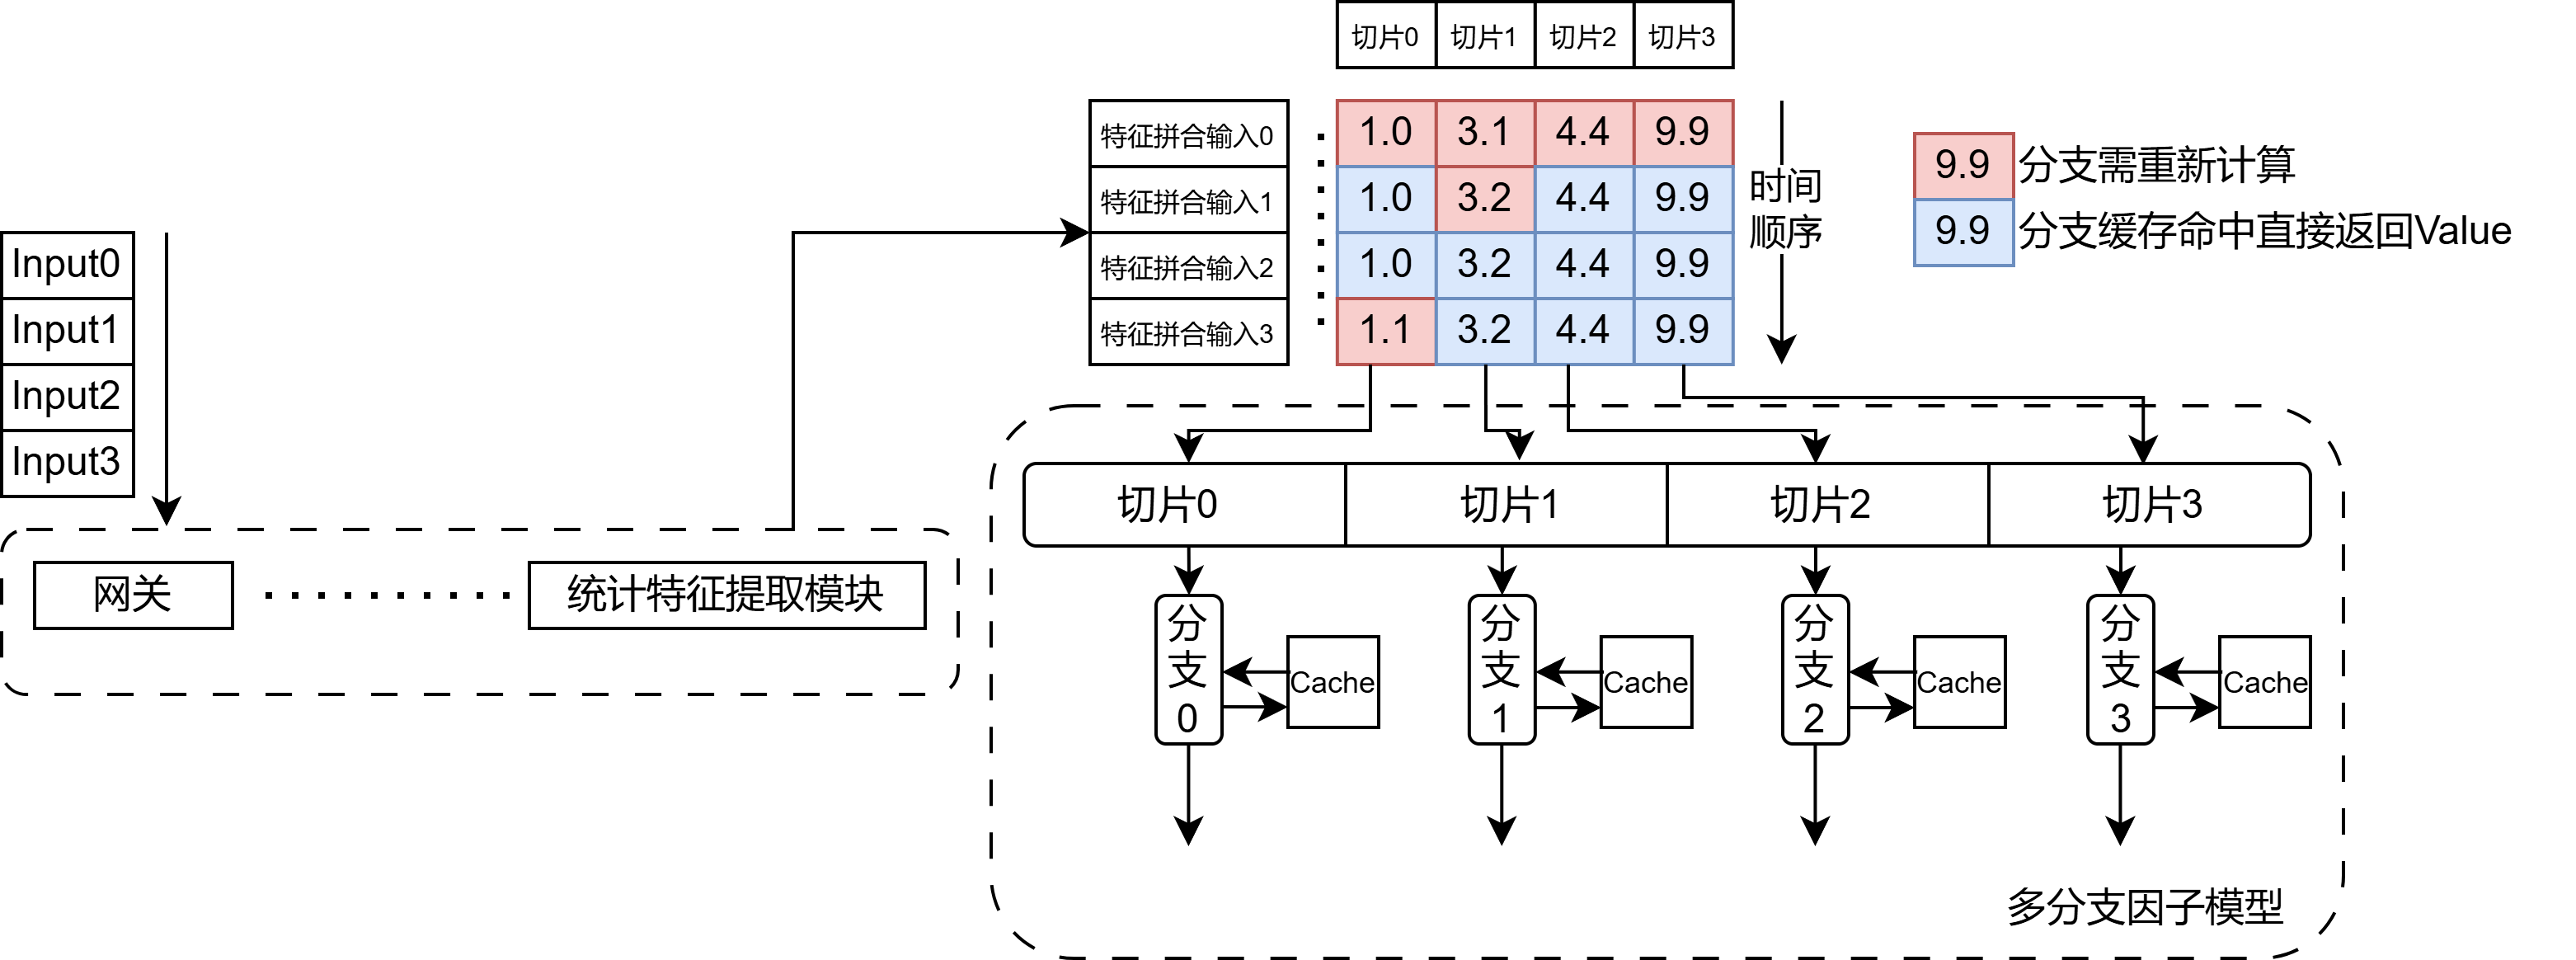
\includegraphics[width=1\textwidth]{image/chap03/high.png}
    \caption{实时行情中缓存加速}
    \label{fig:hole}
\end{figure}


\subsection{基于可枚举输入特征的预计算分支缓存}

以当前成交价格为例,在期货交易市场中,每个交易品类都有一个最小价格波动单位。
除极少的黑天鹅事件外,单个交易日内的价格波动通常在一定范围内。
例如,对于沪铝2503合约,其最小价格波动为5元/吨,而实际交易中单个交易日内价格波动极少超过500元。
基于这一特性,框架通过在盘前预计算并缓存100个波动输入值,为交易日当天所有的成交价格情况做预计算。
这样,在整个交易日内,模型可以直接从缓存中获取这些预计算的值,从而显著减少计算时间。
具体而言,对沪铝2503成交价格的特征输入进行缓存的方法的内存占用较小,通常不多于10KB。
为了实现这一优化,在上述分支拓扑分割算法执行后,框架为每一个分支加入缓存机制。
当市场数据输入与缓存中的数据匹配时,模型直接从缓存中检索预计算的输出,并将其传递给后续节点。
类似的,对于低精度如FP16等数据格式的因子输入,由于多数行情特征为单一值,
因此存在枚举FP16所有取值并预计算分支输出从而建立缓存,将分支推理直接简化为哈希表查询过程的缓存方案。
这不仅减少了冗余计算,还加速了整体的推理过程。
\begin{figure}[h]
    \centering
    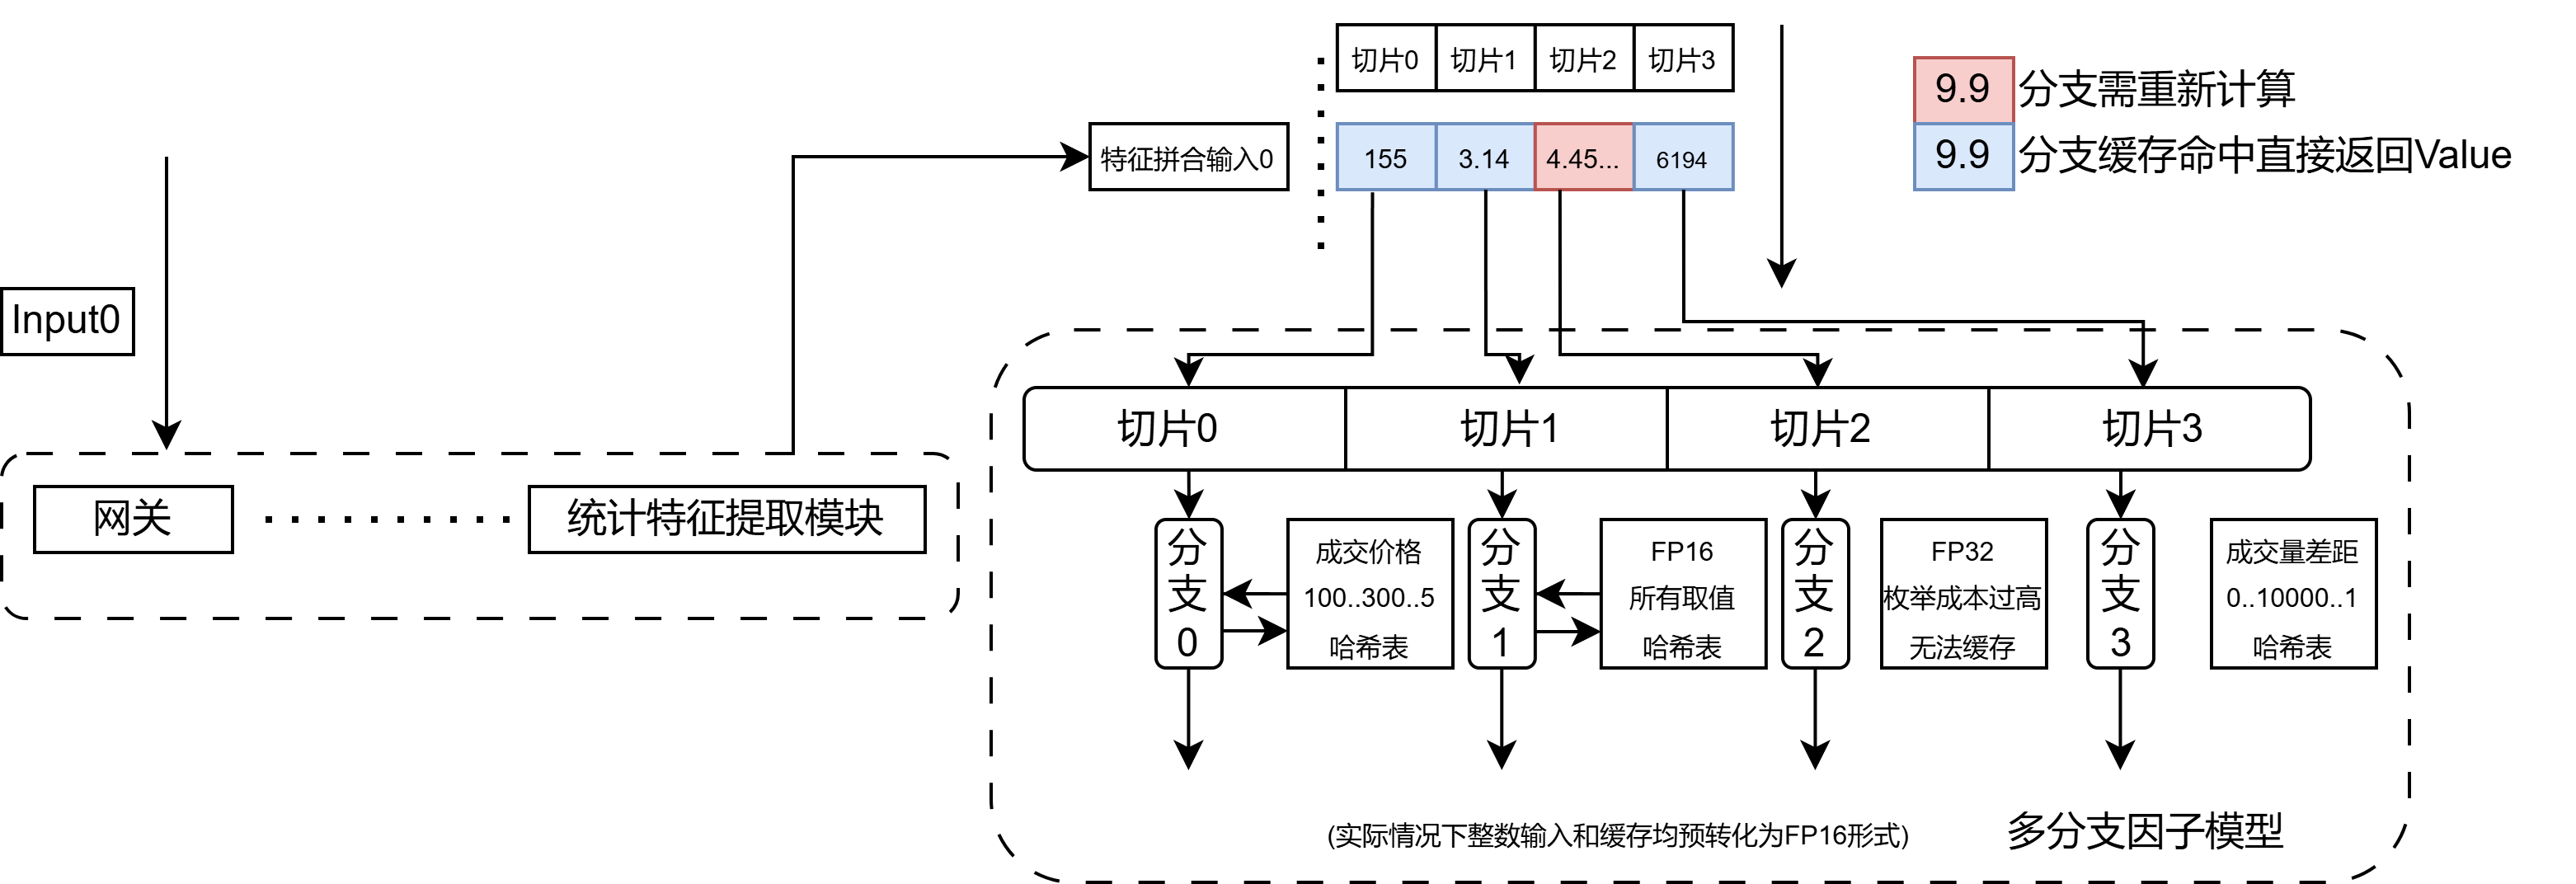
\includegraphics[width=1\textwidth]{image/chap03/precom.png}
    \caption{预计算分支缓存}
    \label{fig:hole}
\end{figure}

\subsection{缓存机制的选取}

实现缓存机制尽管在多数情况下能够实现分支计算过程的简化加速,
但是对于高频交易系统,缓存机制作为分支抽象层的附加实现,需要考虑在缓存未命中条件下的执行延时增加。
而在CPU缓存和系统内存缓存中常用的LRU与FIFO等机制,其需要维护动态缓存池,
相比较匹配上一次输入和预计算固定缓存查询具有较高的延时成本,即便通过维护动态缓存池可能有效提高缓存命中率,但是无缓存命中情况下的推理延时显著增加。
因此缓存机制只使用匹配上一次输入和预计算固定缓存查询两种高效缓存方法,其相比较原推理过程不仅通过缓存命中大幅减少推理延时,在无缓存命中情况下的推理延时几乎没有增加。

综上所述,选择合适的缓存替换机制需要综合考虑市场数据的特性、系统的内存资源以及模型的计算复杂度。
在实际应用中,可以根据具体的交易场景和系统配置,灵活地选择或组合这些缓存策略,以达到最优的性能表现。
在不同的市场条件下,市场数据的特征可能会发生变化,因此需要定期对缓存策略进行评估和调整,以确保其始终能够适应当前的市场环境。
同时,考虑到交易系统的实时性和稳定性要求,缓存机制的实现还需要充分考虑数据的一致性和准确性,避免因缓存数据的错误或过时而导致交易决策的失误。
此外,随着交易规模的扩大和市场数据量的增加,缓存机制的扩展性和可维护性也变得尤为重要,需要在系统设计阶段就充分考虑这些因素,以保证交易系统的长期稳定运行和高效性能。
\newclearpage
\chapter{实验结果与分析}
\label{cha:04}

本章节将对本文提出的多分支因子模型推理框架进行测试与分析,并与当前流行的推理框架Pytorch JIT和计算图推理引擎OnnxRuntime进行推理延时对比。

本章主要内容如下: 
实验环境设置方面,本节介绍了测试使用的样例模型以及测试所使用的软硬件环境等实验准备工作。
数据实验结果展示方面,本节将测试在上述实验环境下样例模型在多分支因子模型推理框架下的性能表现,并与Pytorch JIT\cite{paszke2019pytorchimperativestylehighperformance}和OnnxRuntime进行横向比较。
实验将在预设实验环境下部署本文提出的多分支因子模型推理框架,针对实时行情的不同输入和不同推理框架进行了横向和纵向的性能比较与分析。

\section{实验环境设置}
\label{cha:041}
测试中使用的实验平台, 硬件所使用的CPU为的AMD EPYC 9654 CPU。
在测试数据方面,实验基于2021年9月30日交易日全天沪铝2505的Full Tick交易数据。
在测试模型方面上,实验仍然以\autoref{fig:models}为样例输入模型的示意图。
测试时,实验使用RDTSCP实现基于CPU指令计数器的高精度纳秒计时。 
\autoref{tab:041}中为测试时软硬件环境的详细配置。

\begin{table}[h] %voc table result
    \centering
    \caption{实验环境中的软硬件参数}
    \begin{tabular}{|c|c|}
        \toprule
        \textbf{类型} & \textbf{版本与型号参数} \\
        \midrule
        libprotoc & 3.21.12\\
        \midrule
        Blaze & 3.5\\
        \midrule
        Pytorch & 2.1\\
        \midrule
        Onnx Runtime & 1.21.0\\
        \midrule
        Intel Oneapi & 2025.0\\
        \midrule
        CPU 型号 & AMD EPYC 9654  \\
        \midrule
        C++编译器 & GCC 13.2\\
        \midrule
        性能分析工具 & RDTSCP\\
        \midrule
        操作系统信息 & Ubuntu 24.04 LTS \\
        % \midrule
        \bottomrule
    \end{tabular}
    \label{tab:041}
\end{table}

\section{实验结果与分析}
在高频交易业务场景下,不仅仅需要考虑最大加速效果,而且应当保证在条件机制无效的情况下,附属的动态优化措施本身的执行时间对模型推理的延时影响有限。

而分支缓存机制作为一种高效的过程简化方法,通过将测试样例所得到的延时测算结果进行百分位数排序,从而综合展示分支缓存机制的加速性能和执行过程的高效。

\begin{figure}[h]
    \centering
    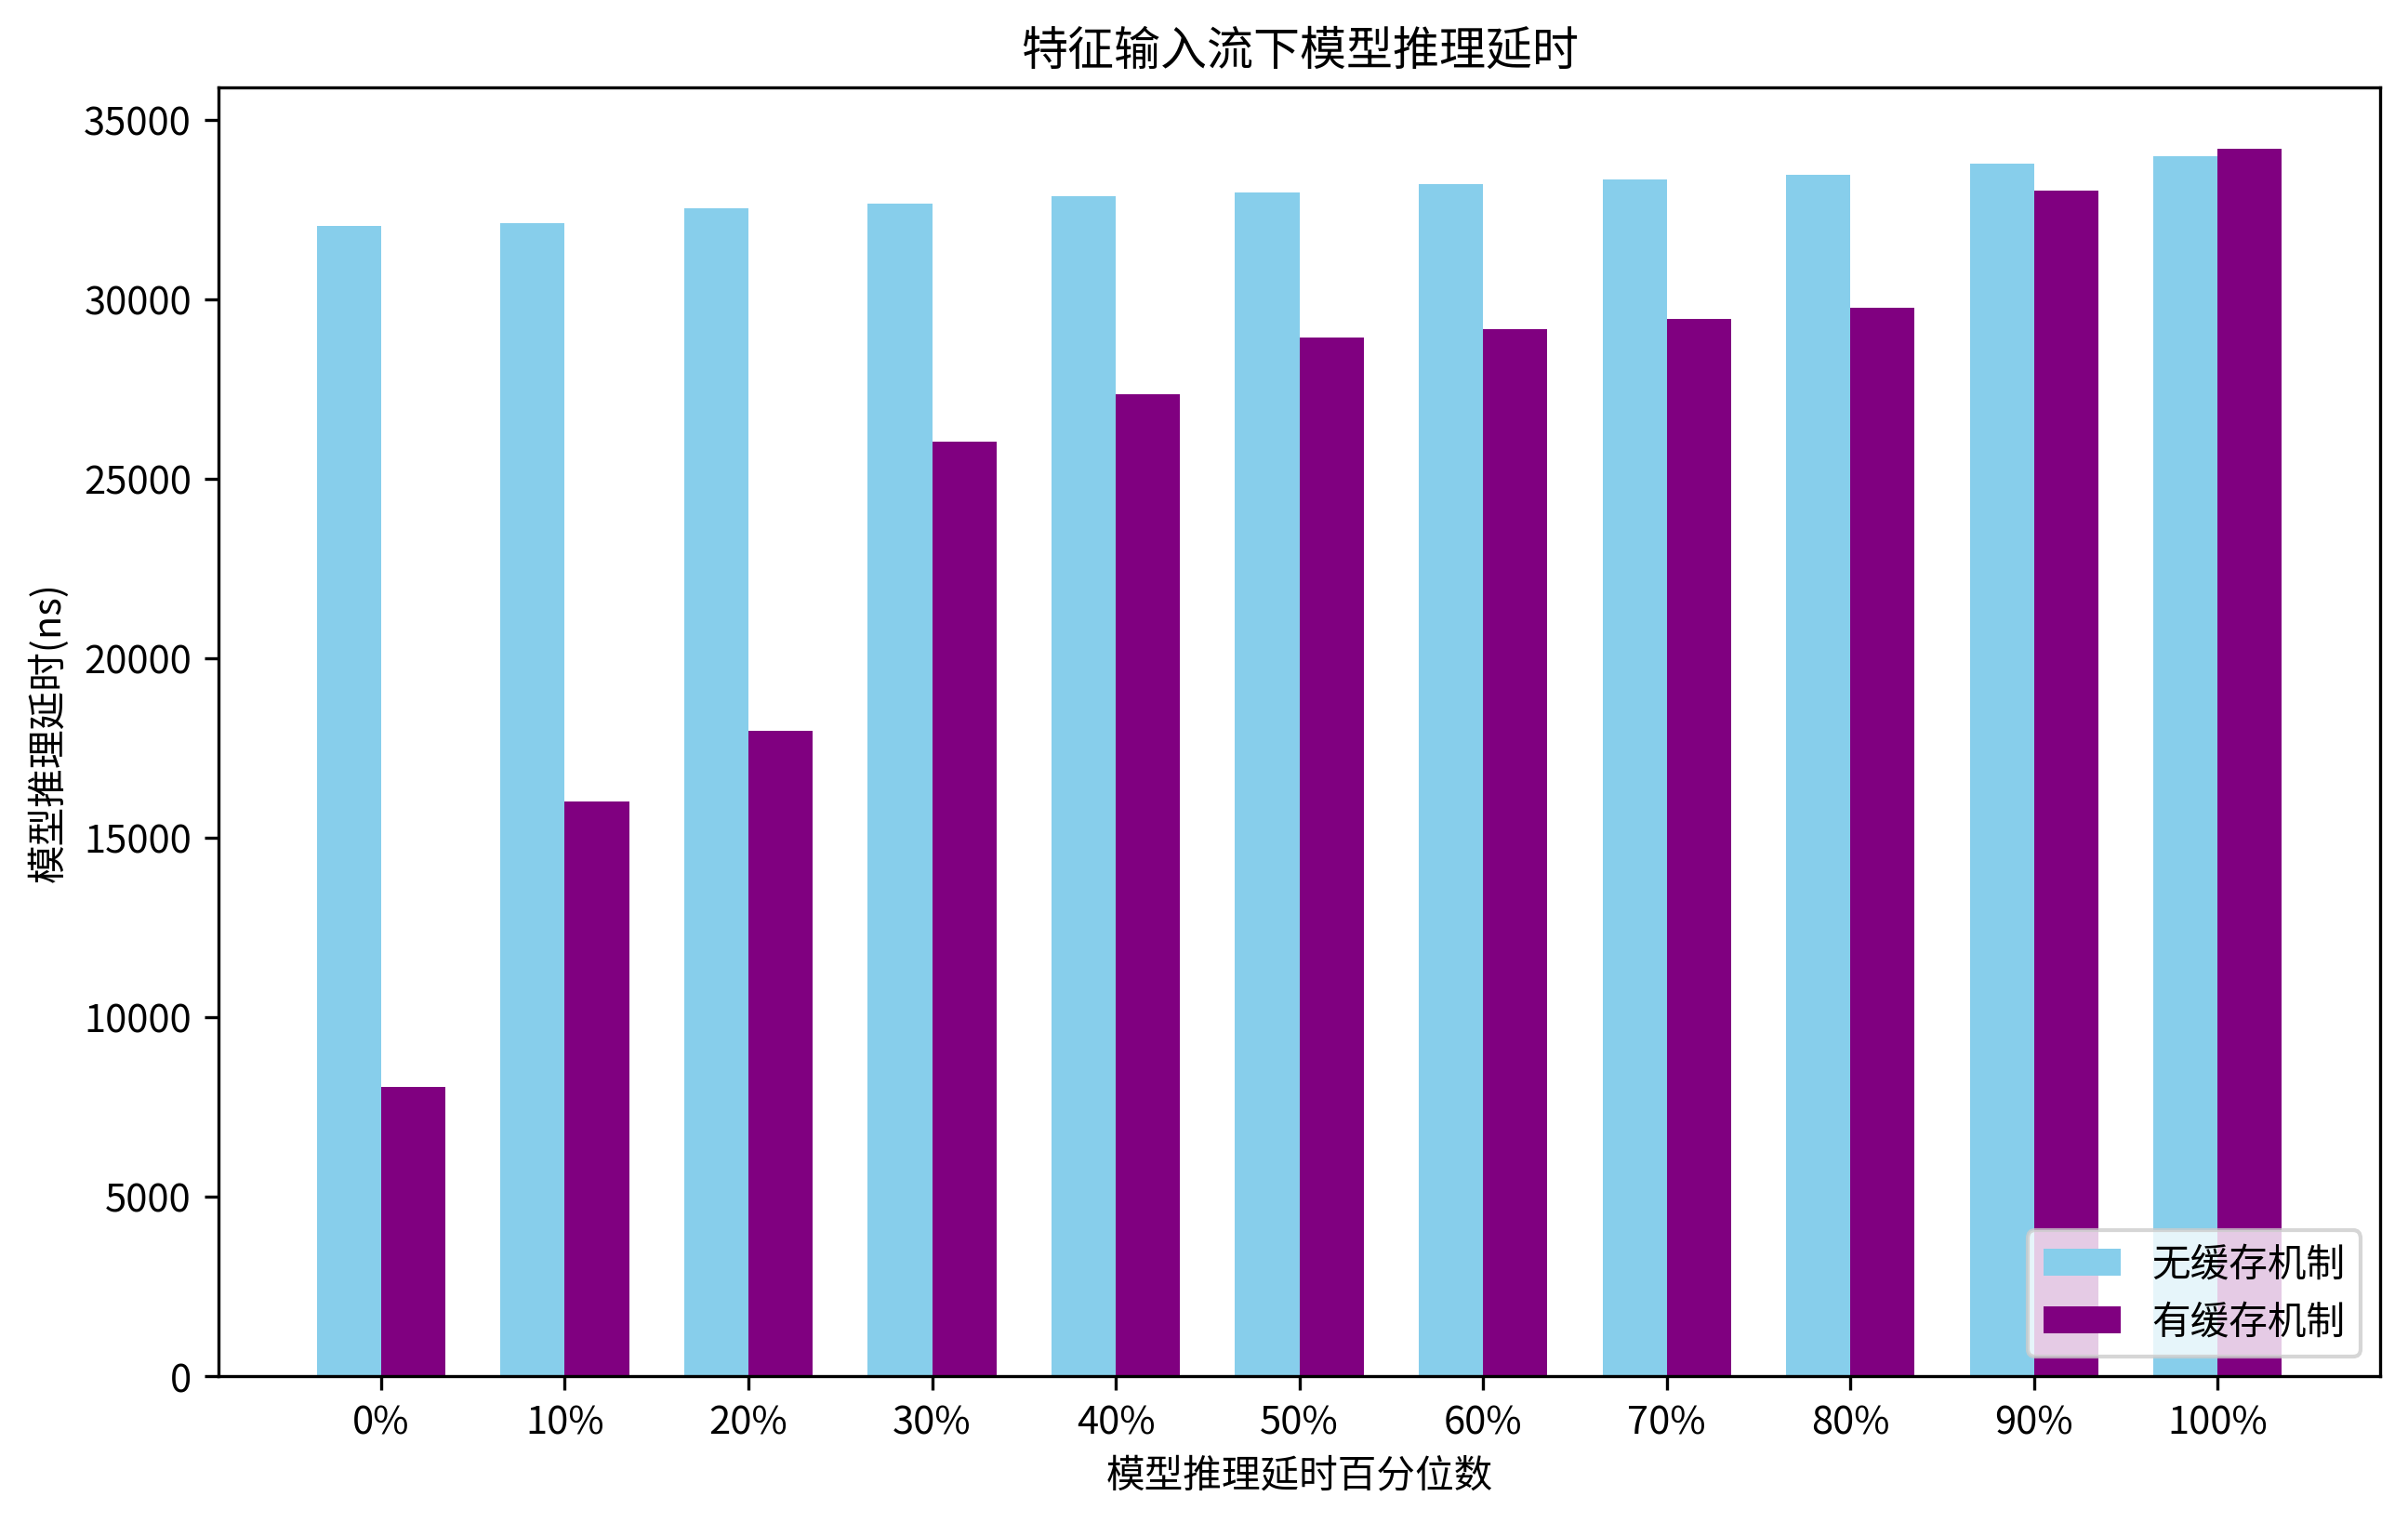
\includegraphics[width=1\textwidth]{image/chap04/outstime.png}
    \caption{启用与不启用缓存机制下测试样例的延时百分位数}
    \label{fig:hole}
\end{figure}

如图所示,在最大延时部分,观察到启用缓存机制后的延时与未启用时的延时基本一致,可以验证分支缓存机制本身执行过程的高效。
证明了仅仅通过输入匹配和预计算哈希表查询对于多分支因子模型的整体推理延时没有显著增长。
同时,观察到启用缓存机制在低延时交易系统更新行情后的多数情况下都表现出缓存命中带来的显著加速,尤其是对于连续特征输入一致的情况下,切片输入分支的后续融合分支也将产生命中从而极大减小计算量综合产生更显著的加速效果。

\begin{figure}[h]
    \centering
    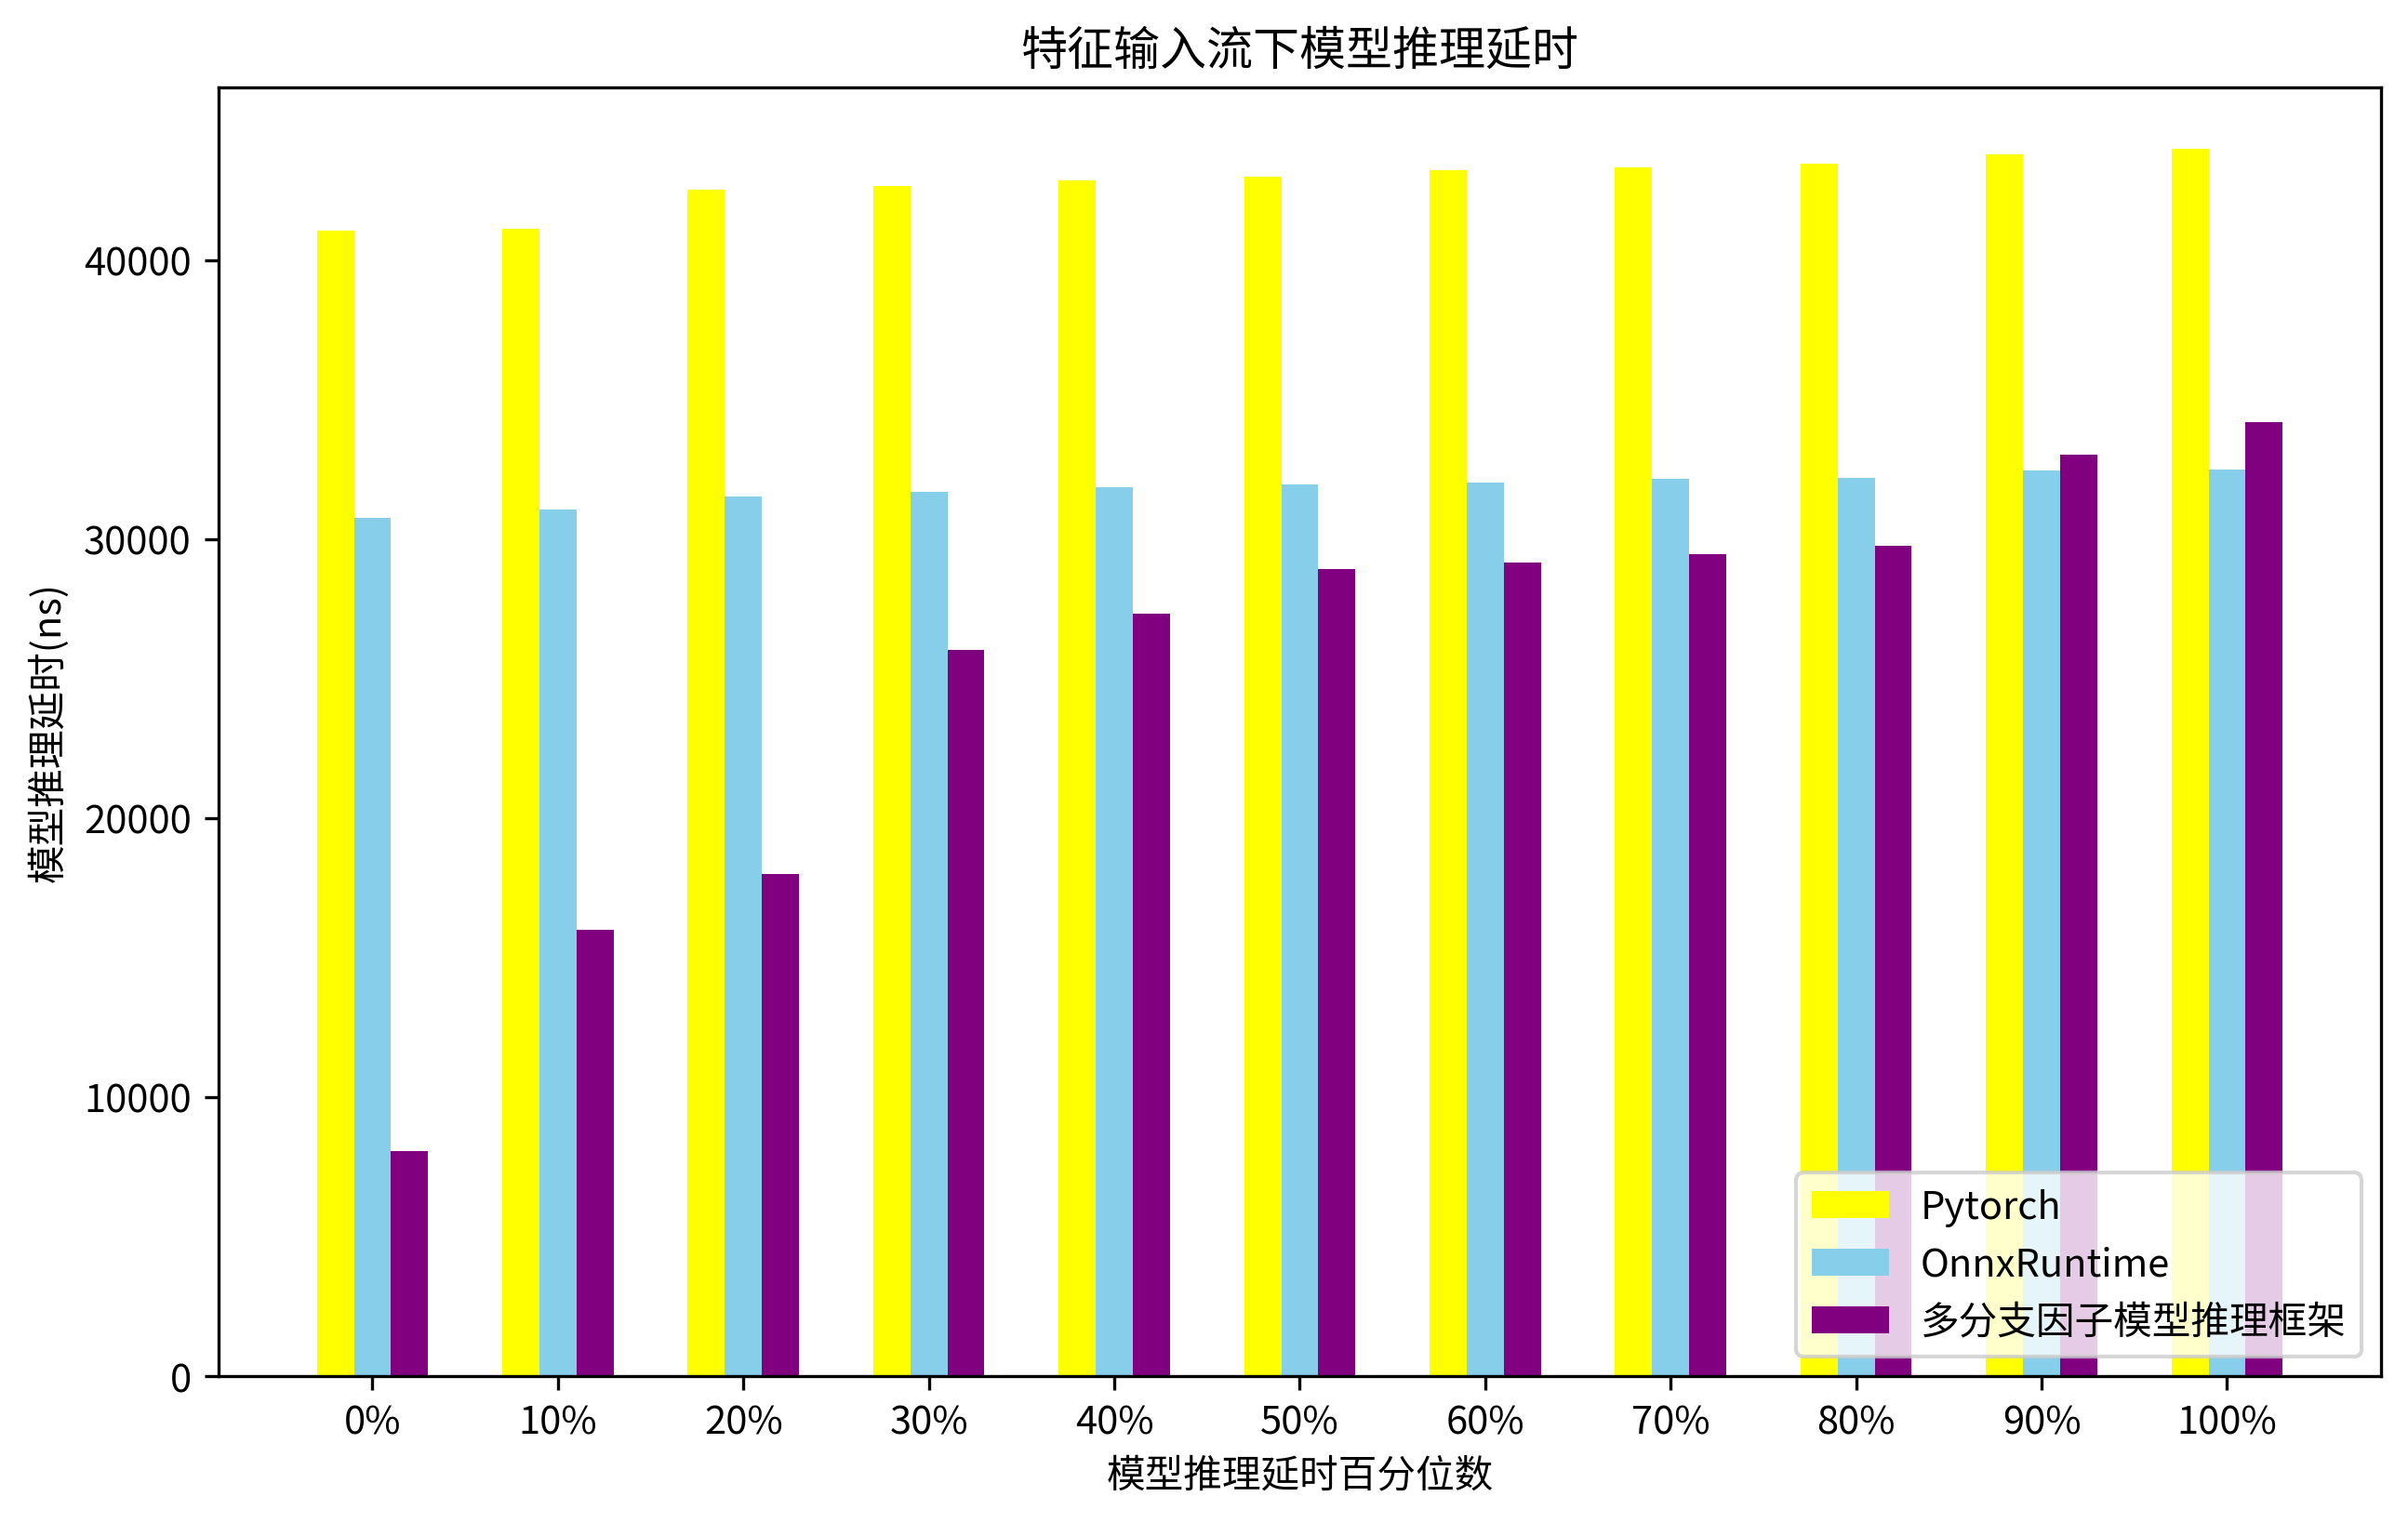
\includegraphics[width=1\textwidth]{image/chap04/outsframe.png}
    \caption{不同推理框架下测试样例的延时百分位数}
    \label{fig:hole}
\end{figure}

如图所示,在最大延时部分,观察到启用缓存机制后模型推理框架推理延时和Onnx Runtime推理延时显著快于Pytorch JIT。
这代表本文提出的多分支因子模型推理框架作为一个轻量级的专用推理框架本身的基础推理性能较好,这也表现出推理框架在计算图方面静态优化带来的显著性能提升。
同时,尽管在该部分Onnx Runtime推理延时略快于本文提出的多分支因子模型推理框架,但是注意到仅在最大延时部分也就是缓存完全未命中时Onnx Runtime才具有此优势,
因此可以通过在项目中加入输入缓存检查从而在无缓存命中时选择Onnx Runtime推理后端以减小最大延时,从而在最大延时情况下利用Onnx Runtime提高推理效率。

另一方面,注意到在发生缓存命中时,本文提出的多分支因子模型推理框架显著降低了推理延时。框架相较于Pytorch JIT实现了从1.28倍到5.09倍的加速,相比较Onnx Runtime实现了从 1.08 倍到 3.82 倍的推理性能提升,相较于Pytorch JIT和Onnx Runtime均具有显著的加速优势。
从而说明分支中的输入匹配和预计算哈希表查询机制在Full Tick行情下具有优越的性能。

\newclearpage
%% chapter 5 dataset, network structure, experiment and result
\chapter{总结与展望}
\label{cha:experiment}

\section{本文工作总结}
本文对高频交易场景的业务特征和多分支因子模型的输入模式与结构特征进行分析,在此基础上设计和实现了一个具有高可拓展性与过程解耦合的因子模型推理框架。
本文在这一推理框架下设计了更详细的加速方案:
首先是利用系统机制有效消除缺页中断和提高访存速度的内存管理方法;
其次设计了针对CPU架构完成算子调优的工作流,并实现了动态算子绑定的拓展机制;
最后,框架充分利用了分支输入的可重复性,实现了基于多分支因子模型的分支划分算法和缓存机制。
实验证明,通过选取恰当的缓存方法,框架相较于Pytorch JIT实现了从1.28倍到5.09倍的加速,相较于Onnx Runtime实现了从1.08倍到3.82倍的加速


\section{讨论和展望}
尽管本文提出的框架方案相较已有相关工作显著降低了延时,但仍存在许多需要改进的方面。本小节将概述本文工作的不足与局限,并展望未来的研究方向。

首先,针对多分支因子模型的结构特征,仍然可能存在进一步的优化空间,多分支结构的分支之间互相独立,因此各分支的推理过程存在线程并行的加速空间。
同时考虑到并行线程面向不同CPU架构时存在核心绑定相关调优问题,因此亟待进一步开发与研究。

其次,系统友好的内存管理方案和硬件友好的算子调优和动态绑定方案仍然具有优化空间。
当前推理进程仍然运行在操作系统用户态,仍然存在大量无关进程影响交易系统运行,
理想情况下,应当使整个交易链路直接运行在内核态从而最大限度减少由于系统调用中断导致的延时。

最后,尽管本文提出和实现了一个过程解耦和具有高可拓展性的因子模型推理框架,但是当前的研究仅仅局限于针对多分支因子模型的特性设计和实现优化算法。
伴随着量化交易的进一步发展,当前的优化方法很可能不再适用于具有更优性能的不同结构因子模型,本文提出的方案仍然需要进一步的开发研究。

\newclearpage

% 结语

% 附录部分
\backmatter
% 参考文献. 因不需要纳入章节目录, 故放入附录部分
% 实际上参考文献是属于论文主体部分
\makereferences

% 附录
% {
%     \appendix
%     %\chapter{补充更多细节}

\section{补充图}

\subsection{补充图}

这是附录内容,应该用宋体小四号字体。


\endinput

%     \newclearpage
% }

%%
% 致谢
% 谢辞应以简短的文字对课题研究与论文撰写过程中曾直接给予帮助的人员(例如指导教师、答疑教师及其他人员)表示对自己的谢意,这不仅是一种礼貌,也是对他人劳动的尊重,是治学者应当遵循的学术规范。内容限一页。
% modifier: 黄俊杰
% update date: 2017-04-15
%%

\chapter{致谢}

四年时光如白驹过隙,本科求学之路随之画上句点。回首往昔,我深感这段时光不仅丰富了我的知识与技能,提高了我的科学素养,更培养了我分析问题、解决问题的能力和不畏困难、深度求索的精神。
就读于中山大学的宝贵经历是我永久的财富。在此,我想衷心感谢那些给予我帮助与支持的老师、家人和同学们。

首先,我要特别感谢我的指导老师卢宇彤教授。作为一名本科生,我缺乏学术研究的经验,难以准确把握研究问题的要点,也难以评估自己的工作水平。而卢老师对所涉领域有着深刻的理解,她的广博知识和敏锐洞察力给予了我宝贵的指导。卢老师严谨的治学态度和勤奋的工作精神更是我学习的楷模。在此,我向卢老师致以崇高的敬意和诚挚的感谢。

其次,我要感谢我的家人。在我面临困难和挑战时,他们给予了我无私的支持与鼓励,让我坚持不懈、保持信心。正是因为他们的支持和付出,我才能够坚定不移地追求目标,在求学进步的道路上笃定前进。

最后,我要感谢所有曾经帮助过我的朋友们。你们的热心支持与耐心鼓励永远是我前行路上最坚实的后盾,我会倍加珍惜这份情谊,不忘初心,继续前行。

\vskip 108pt
\begin{flushright}
	卢科州\makebox[1cm]{} \\
	\today
\end{flushright}

    % 致谢
\newclearpage

% \makeGrade      % 成绩评定记录表
\end{document}
